\documentclass[12pt]{article}

% ---------------------------------------------------------------------------
% Detection Without Identification: ShotSpotter and Gun Homicide in Chicago
% ACE 592 Final Project -- Austin Belman and Kameron Nelson
% Built from NARRATIVE.md and the analysis pipeline in this repository.
% Compile: pdflatex final_paper.tex  (run twice for cross-references)
% ---------------------------------------------------------------------------

\usepackage[T1]{fontenc}
\usepackage[utf8]{inputenc}
\usepackage[margin=1in]{geometry}
\usepackage{mathptmx}            % Times-like serif
\usepackage{microtype}           % better justification; eliminates most overfull boxes
\usepackage{setspace}
\usepackage{graphicx}
\graphicspath{{../plots/}}
\usepackage{booktabs}
\usepackage{amsmath}
\usepackage{array}
\usepackage{float}
\usepackage{caption}
\captionsetup{font=small,labelfont=bf,justification=raggedright,singlelinecheck=false}
\usepackage[hidelinks]{hyperref}

\setlength{\parindent}{0.5in}
\setlength{\parskip}{0pt}

% Tighter, readable tables
\renewcommand{\arraystretch}{1.15}

\title{\vspace{-1.5em}\textbf{Detection Without Identification:\\
ShotSpotter and Gun Homicide in Chicago, 2009--2023}}
\author{Austin Belman and Kameron Nelson\\
\small University of Illinois Urbana--Champaign\\
\small ACE 592 Final Project}
\date{}

\begin{document}

\maketitle
\thispagestyle{empty}

% ===========================================================================
\begin{abstract}
\noindent
Between 2017 and 2023, Chicago paid millions of dollars to deploy ShotSpotter---an
acoustic gunshot-detection system---across 51 of its 77 community areas, and Mayor
Brandon Johnson cancelled the contract in 2023 citing limited evidence of impact. That
ShotSpotter does not reduce gun violence is by now well established---in Chicago at the
police-district level (Connealy et al., 2024) and nationally (Doucette et al., 2021); the
question we take up is not whether that null replicates but whether the public,
community-area-level data that anchor most policy debate can \emph{identify} a causal
effect at all. Using a community-area-by-year panel of gun homicides spanning 2009--2023,
we estimate five classes of model: (i) a two-way fixed-effects OLS difference-in-differences
(DiD); (ii) Poisson and Negative Binomial regressions appropriate for count outcomes;
(iii) cohort-specific and Callaway--Sant'Anna (2021) event studies that respect the
staggered 2017/2018 rollout; (iv) a synthetic control with permutation inference; and (v)
pre-period placebo tests. The OLS DiD coefficient is positive and significant ($\beta =
+2.63$ gun homicides per area-year, $p < 0.001$) and survives unit and year fixed
effects---but it is a count-data misspecification artifact (Silva \& Tenreyro, 2006):
estimated as Poisson or Negative Binomial with the same fixed effects, the effect
collapses to a statistically null incidence-rate ratio of $\approx 1.07$ ($p \approx
0.5$), with confidence intervals spanning anywhere from a 13\% reduction to a 33\%
increase. The design also fails a joint parallel-trends Wald test ($F = 19.9$, $p =
0.006$), produces similarly ``significant'' coefficients when treatment is faked in
pre-rollout years, and admits no feasible synthetic control because the 26 never-treated
areas are systematically lower-violence than any treated neighborhood. A placement model
makes the selection explicit: ShotSpotter siting is predicted by structural disadvantage
and pre-period violence with near-perfect separation (propensity AUC $0.94$), and the six
highest-violence study neighborhoods have no comparably situated untreated counterpart.
These data therefore \emph{cannot identify} a causal effect of ShotSpotter on gun
homicides in either direction. They rule out a large \emph{deterrence} effect, but cannot
exclude the survival-channel mortality benefit that a boundary regression discontinuity
attributes to faster emergency response---a magnitude that lies inside our confidence
interval and that this design is not built to detect. The contribution is thus a worked
identification-limits case: a coefficient can survive fixed effects and robustness
restrictions and still fail every condition a causal reading requires.
\end{abstract}

\doublespacing

% ===========================================================================
\section{Introduction}

Gun violence in the United States is a persistent public-health crisis that
disproportionately affects young people of color and is heavily concentrated in large
metropolitan areas (CDC, 2020; Kegler, Dahlberg, \& Mercy, 2018). One barrier to reducing
firearm violence is the chronic underreporting of gunfire: research finds that only about
20\% of shootings are reported to law enforcement (Irvin-Erickson et al., 2016; Carr \&
Doleac, 2016). In response, cities have turned to
gunshot-detection technology---most notably ShotSpotter---to close that measurement gap
and improve real-time awareness of gunfire (Choi, Librett, \& Collins, 2014). This paper
uses Chicago's deployment of that technology not to re-evaluate it, but to ask what the
public data most policy debate relies on can---and cannot---identify.

Chicago piloted ShotSpotter in 2012 in two small zones, expanded to full district
coverage in 2016, and signed a three-year, \$3 million contract to widen coverage in
2018 (Office of Inspector General, 2021). The system has been controversial: a 2021
Office of Inspector General (OIG) audit found that alerts rarely produced evidence used
in investigations; advocacy groups argued the technology concentrated police presence in
already over-policed Black and Brown communities; and in 2023 Mayor Brandon Johnson
terminated the contract, citing reliability and community-impact concerns.

The empirical question that motivated ShotSpotter is straightforward---\emph{did it reduce
gun violence?}---and for Chicago it is largely answered. A matched quasi-experiment of the
technology's staggered rollout across Chicago police districts finds no reduction in fatal
or non-fatal shootings, gun crimes, or shots-fired calls, only a rise in recovered
evidence (Connealy et al., 2024); a national panel of large metropolitan counties reaches
the same null for firearm homicides and arrests (Doucette et al., 2021); and a
district-level study finds that, if anything, the technology slowed dispatch and lowered
arrest probability (Topper \& Ferrazares, 2024). Replicating that null is not this paper's
contribution. What no prior evaluation has done is run the design at the community-area
level---the 77-unit geography in which Chicago's open data are published and its policy
debate is conducted, finer than the police districts of the existing Chicago evaluations
(Connealy et al., 2024; Topper \& Ferrazares, 2024).

Our question is instead a methodological one: can the public, community-area-level data
that dominate policy debate \emph{identify} such an effect at all, and what happens when a
conventional evaluation is run on them without asking? The answer, defensibly stated, is
that \textbf{no design we can run produces a credible causal estimate}---and the
instability is diagnostic, not incidental. It is the signature of a research design with no
valid control group and a pre-period dominated by a single anomalous year. Three findings
organize the paper. First, a standard two-way fixed-effects DiD manufactures a large,
significant, robustness-surviving positive coefficient that collapses to a null the moment
the count outcome is modeled correctly (Silva \& Tenreyro, 2006; Wilson, 2022)---a worked
instance, on a live \$3 million procurement decision, of a coefficient that passes every
routine check yet fails a causal reading (LaLonde, 1986). Second, we estimate the selection
mechanism the design founders on: ShotSpotter placement is predicted by structural
disadvantage and prior violence so tightly that the highest-violence treated neighborhoods
have no comparably situated untreated counterpart, which is what makes a synthetic control
literally non-constructible rather than merely imperfect. Third, we state the substantive
envelope honestly: the data rule out a large \emph{deterrence} effect but cannot exclude a
survival-channel mortality benefit of the kind a boundary regression discontinuity
attributes to faster response---a magnitude that falls inside our own confidence interval.
We close with the conclusion the data robustly support---that ShotSpotter functioned as a
detection instrument, not as a demonstrated violence-reduction intervention---a reading
consistent with the 2023 decision to end the contract.

% ===========================================================================
\section{Background: ShotSpotter in Chicago}

ShotSpotter is a real-time acoustic-detection service. Microphones triangulate the sound
of gunfire, an algorithm filters non-gunshot sounds, and a human acoustic expert reviews
the alert before it is dispatched to police (Choi, Librett, \& Collins, 2014; Gatens \&
Reichert, 2019). The technology is sold as a response-time tool: faster, more accurate
detection should mean faster police response and faster trauma care, and therefore---in
principle---fewer deaths. While some scholars argue that policing and enforcement can
reduce gun violence (Braga \& Cook, 2023), others caution that aggressive enforcement
carries serious social costs for communities already disproportionately affected by
violence (Harcourt, 2019; Raphael \& Stoll, 2013).

The evaluation record on gunshot detection is, by now, fairly settled, and it splits along
one seam: the technology reliably improves \emph{process} outcomes---faster detection, more
ballistic evidence, fewer shots-fired calls---but not the \emph{victim} outcomes that
motivate its purchase. A microsynthetic-control evaluation in Kansas City draws the seam
sharply (Piza et al., 2024): coverage raised ballistic-evidence collection and cut
shots-fired calls, yet left fatal shootings, non-fatal shootings, and gun assaults
unchanged. Neighborhood evaluations in St.\ Louis echo it---roughly a 25\% drop in citizen
shots-fired calls with no change in violent crime (Mares \& Blackburn, 2021)---while results
elsewhere range from crime reductions (Mares, 2023) to increases coinciding with deployment
(Vovak et al., 2021). The same null holds at coarser units: staggered evaluations across
Chicago police districts (Connealy et al., 2024) and metropolitan counties nationally
(Doucette et al., 2021) find no reduction in shootings, homicides, or case clearance, a
Chicago district study finds detection even slowed dispatch and lowered arrest probability
(Topper \& Ferrazares, 2024), and a 2026 meta-analysis of 44 estimates across eight studies
pools to a null relative incidence-rate ratio of $1.02$ (95\% CI $[0.90, 1.16]$; Huff,
Dunlap, \& Pearson, 2026). The one channel with a credible claim to benefit is medical: a
boundary regression discontinuity attributes a lower shooting-fatality rate inside coverage
to faster emergency response (University of Chicago Crime Lab, 2024, not peer-reviewed). Against that
backdrop, the question this paper takes up is not whether detection deters homicides---the
weight of the evidence says it does not---but whether the community-area data on which most
local policy argument relies can \emph{identify} such an effect at all, and how a routine
evaluation run on those data can mislead.

Chicago's deployment was concentrated in the city's most disinvested neighborhoods. Each
of the six neighborhoods studied here---Austin, Humboldt Park, North Lawndale,
Englewood, West Englewood, and South Shore---has a poverty rate roughly twice the
Chicago average (28.6\%--46.6\% versus 19.7\% city-wide), unemployment 1.5--3 times the
city rate, and a hardship index between 55 and 94 against a city-wide median below 50
(Census 2008--2012). The 51 ShotSpotter community areas accounted for an average of 381
gun homicides per year in 2009--2016, against 42 per year across the 26 community areas
without ShotSpotter---roughly a 9-to-1 ratio in aggregate, and about 4.6 times the
homicides \emph{per area}. That ratio is the central methodological challenge of the
paper: \textbf{ShotSpotter was deployed \emph{because} of concentrated violence and
disadvantage, not assigned at random}---a selection rule we estimate directly in
Section~\ref{sec:placement}. Figure~\ref{fig:map} shows the resulting geography of treatment
and control.

\begin{figure}[H]
\centering
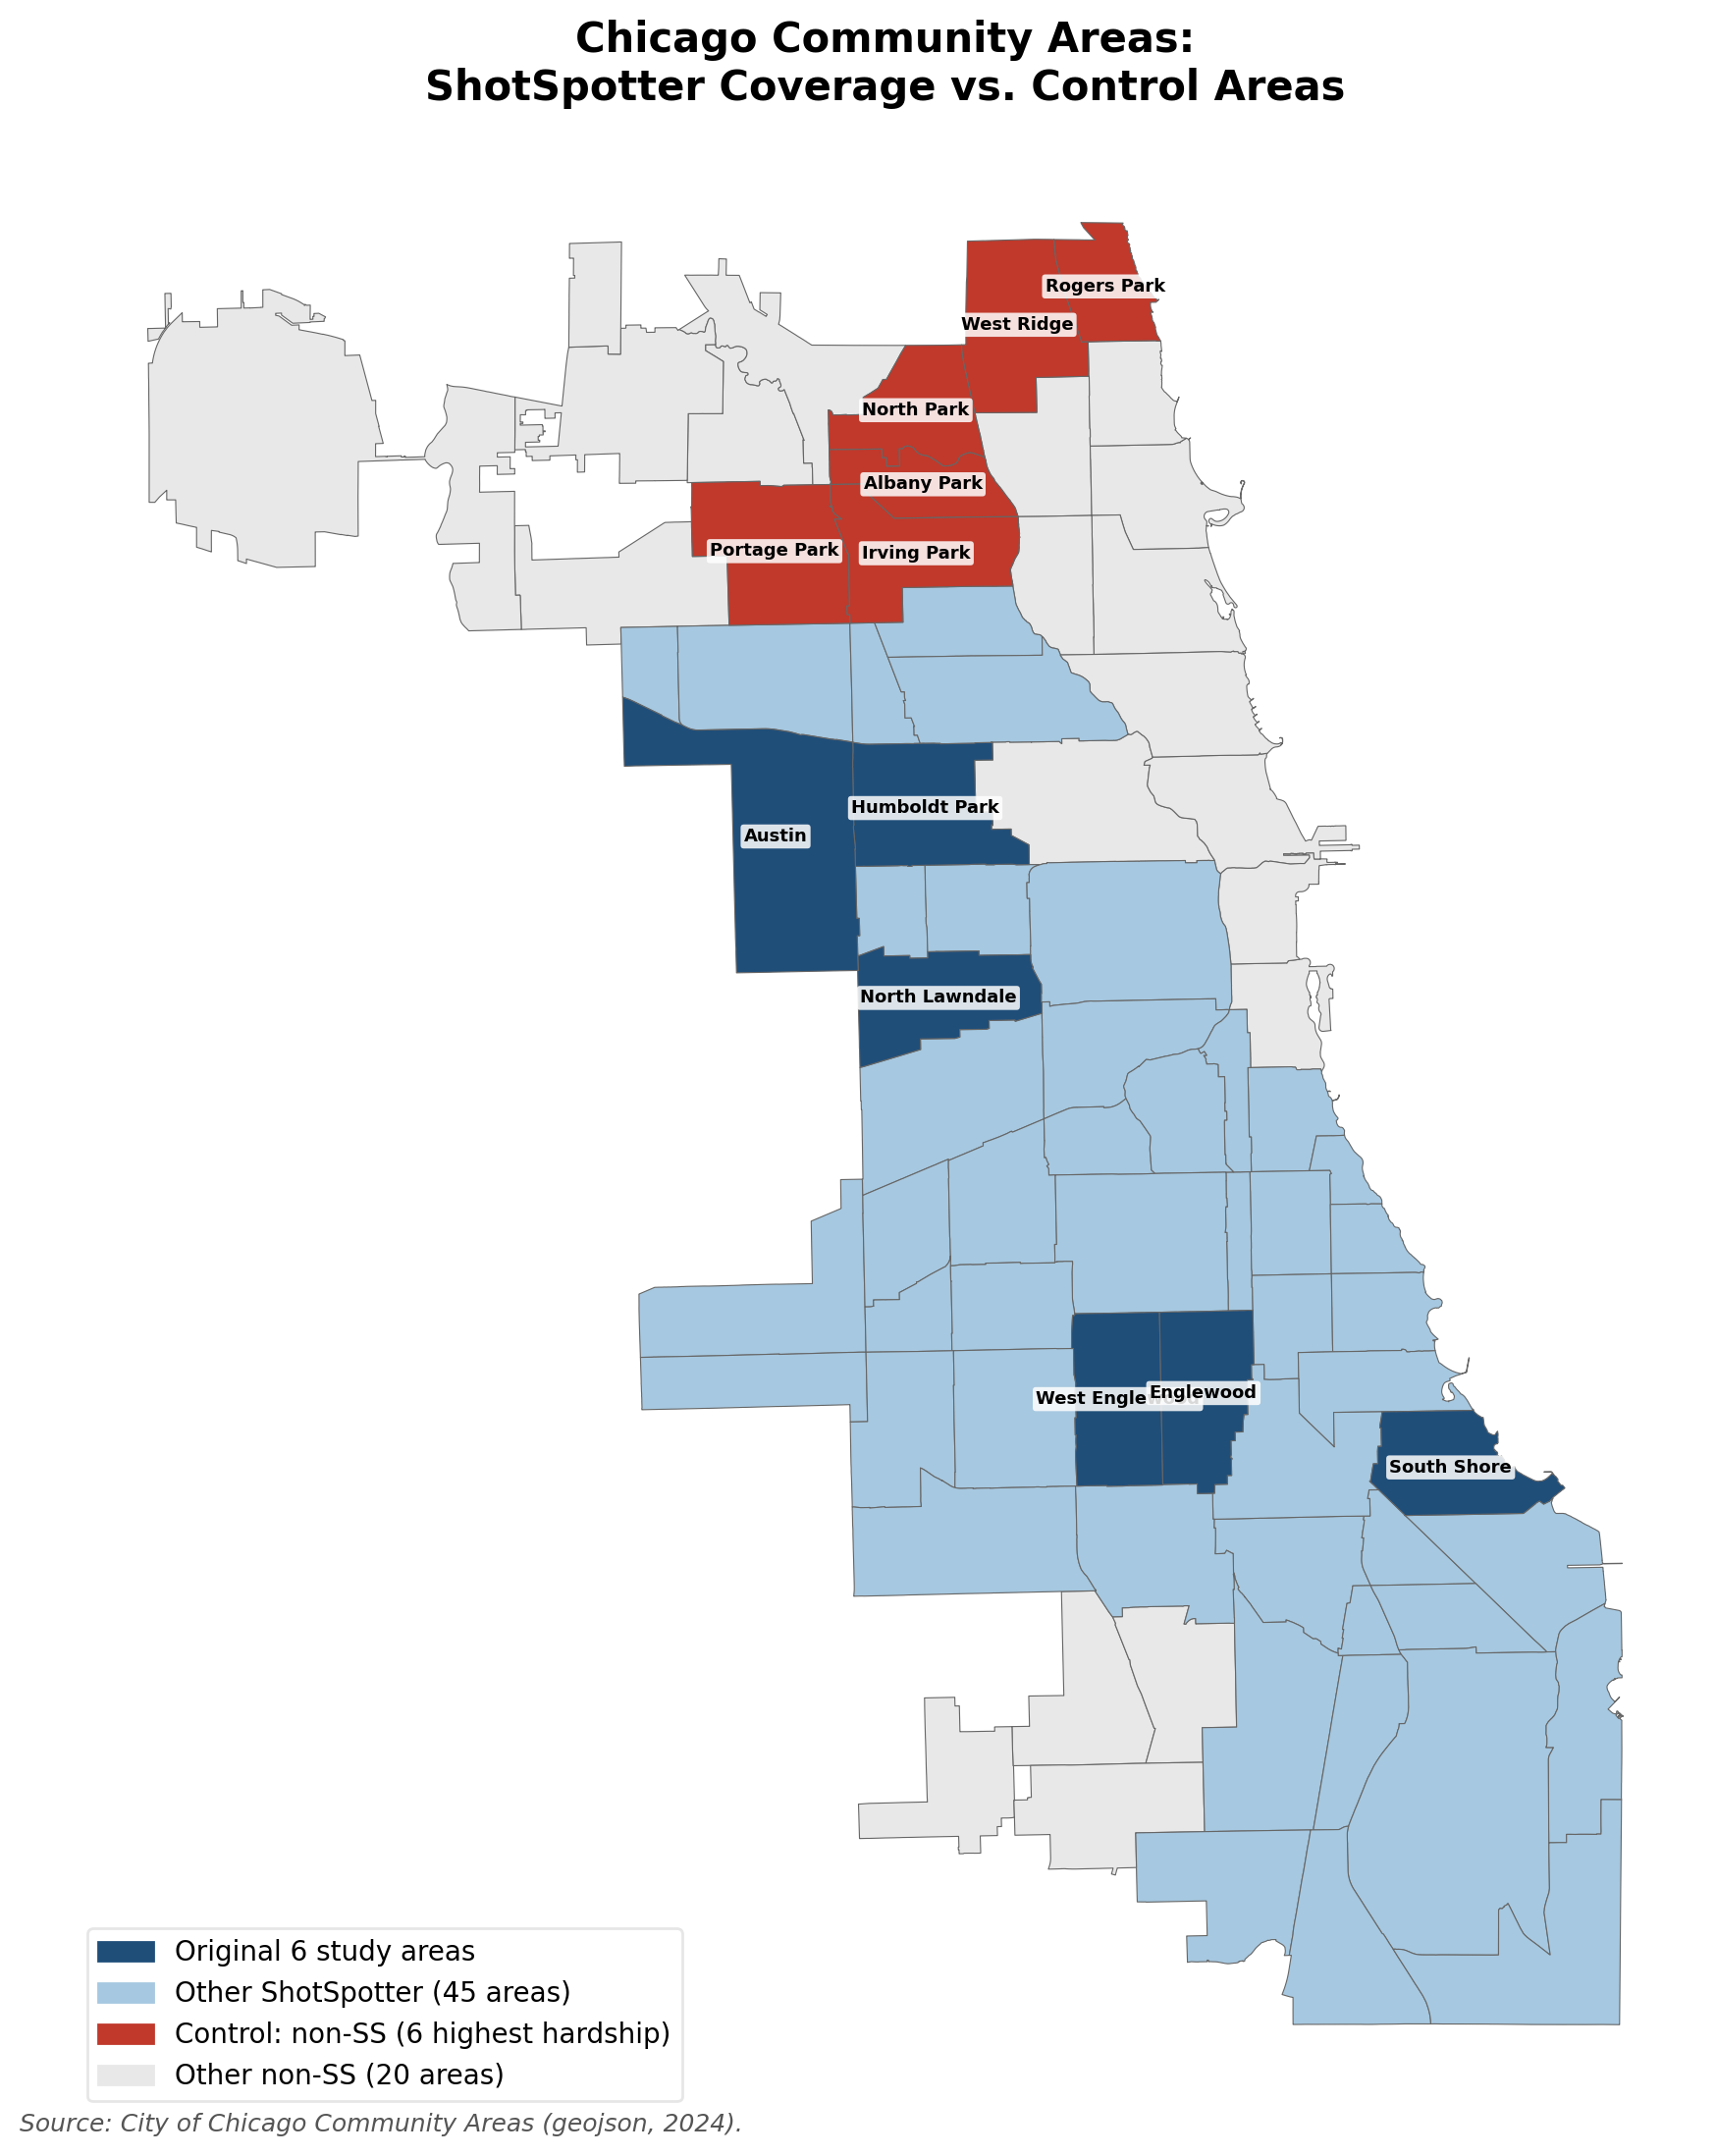
\includegraphics[width=0.72\textwidth]{did_map_treatment_control.png}
\caption{ShotSpotter coverage (treatment, blue) blankets the high-violence South and
West sides; the 26 never-treated community areas form the control group, with the six
highest-hardship ones highlighted in red. Treatment was assigned because of pre-existing
violence, which is the selection problem every design in this paper must confront.}
\label{fig:map}
\end{figure}

% ===========================================================================
\section{Data}

The analysis combines four City of Chicago open-data products, all freely available
from the Chicago Data Portal:

\begin{itemize}
\itemsep0.1em
\item \textbf{Violence Reduction---Victims of Homicides and Non-Fatal Shootings}
(61,450 incidents, 1991--2025), filtered to gun homicides ($n \approx 7{,}600$ in
2009--2023) and non-fatal gunshot injuries ($n \approx 30{,}000$).
\item \textbf{Violence Reduction---ShotSpotter Alerts (Historical)} (222,108 alerts,
2017-01-13 to 2024-09-22, when the city ended ShotSpotter; the 191,824 alerts through 2023
fall in our analysis window).
\item \textbf{Census Data---Selected Socioeconomic Indicators, 2008--2012} (77 community
areas plus the city total).
\item \textbf{Community Areas GeoJSON} (77 polygons).
\end{itemize}

The ShotSpotter dataset reveals the staggered rollout structure that the analysis
exploits: 21 community areas appear in the data beginning in early 2017 and 30 between
mid-2017 and mid-2018, leaving 26 never-treated areas. Treatment status is inferred from
alert presence, so a community area counts as treated when district-level sensor coverage
reached any part of it. The original project pipeline
collapses both cohorts to a single 2017 cutoff---the standard convention, but one that
biases pooled estimates when treatment timing varies (Goodman-Bacon, 2021), motivating
the cohort-aware estimators below. Homicide and alert data are aggregated to the
community-area-by-year (and, for descriptive figures, community-area-by-month) level.

Figure~\ref{fig:comparison} shows the raw before/during homicide comparison for the six
study neighborhoods. Counts rose in most of them---but, as the rest of the paper makes
clear, a raw before/during comparison is exactly the kind of contrast that selection and
the city-wide trend render uninterpretable as a causal effect.

\begin{figure}[H]
\centering
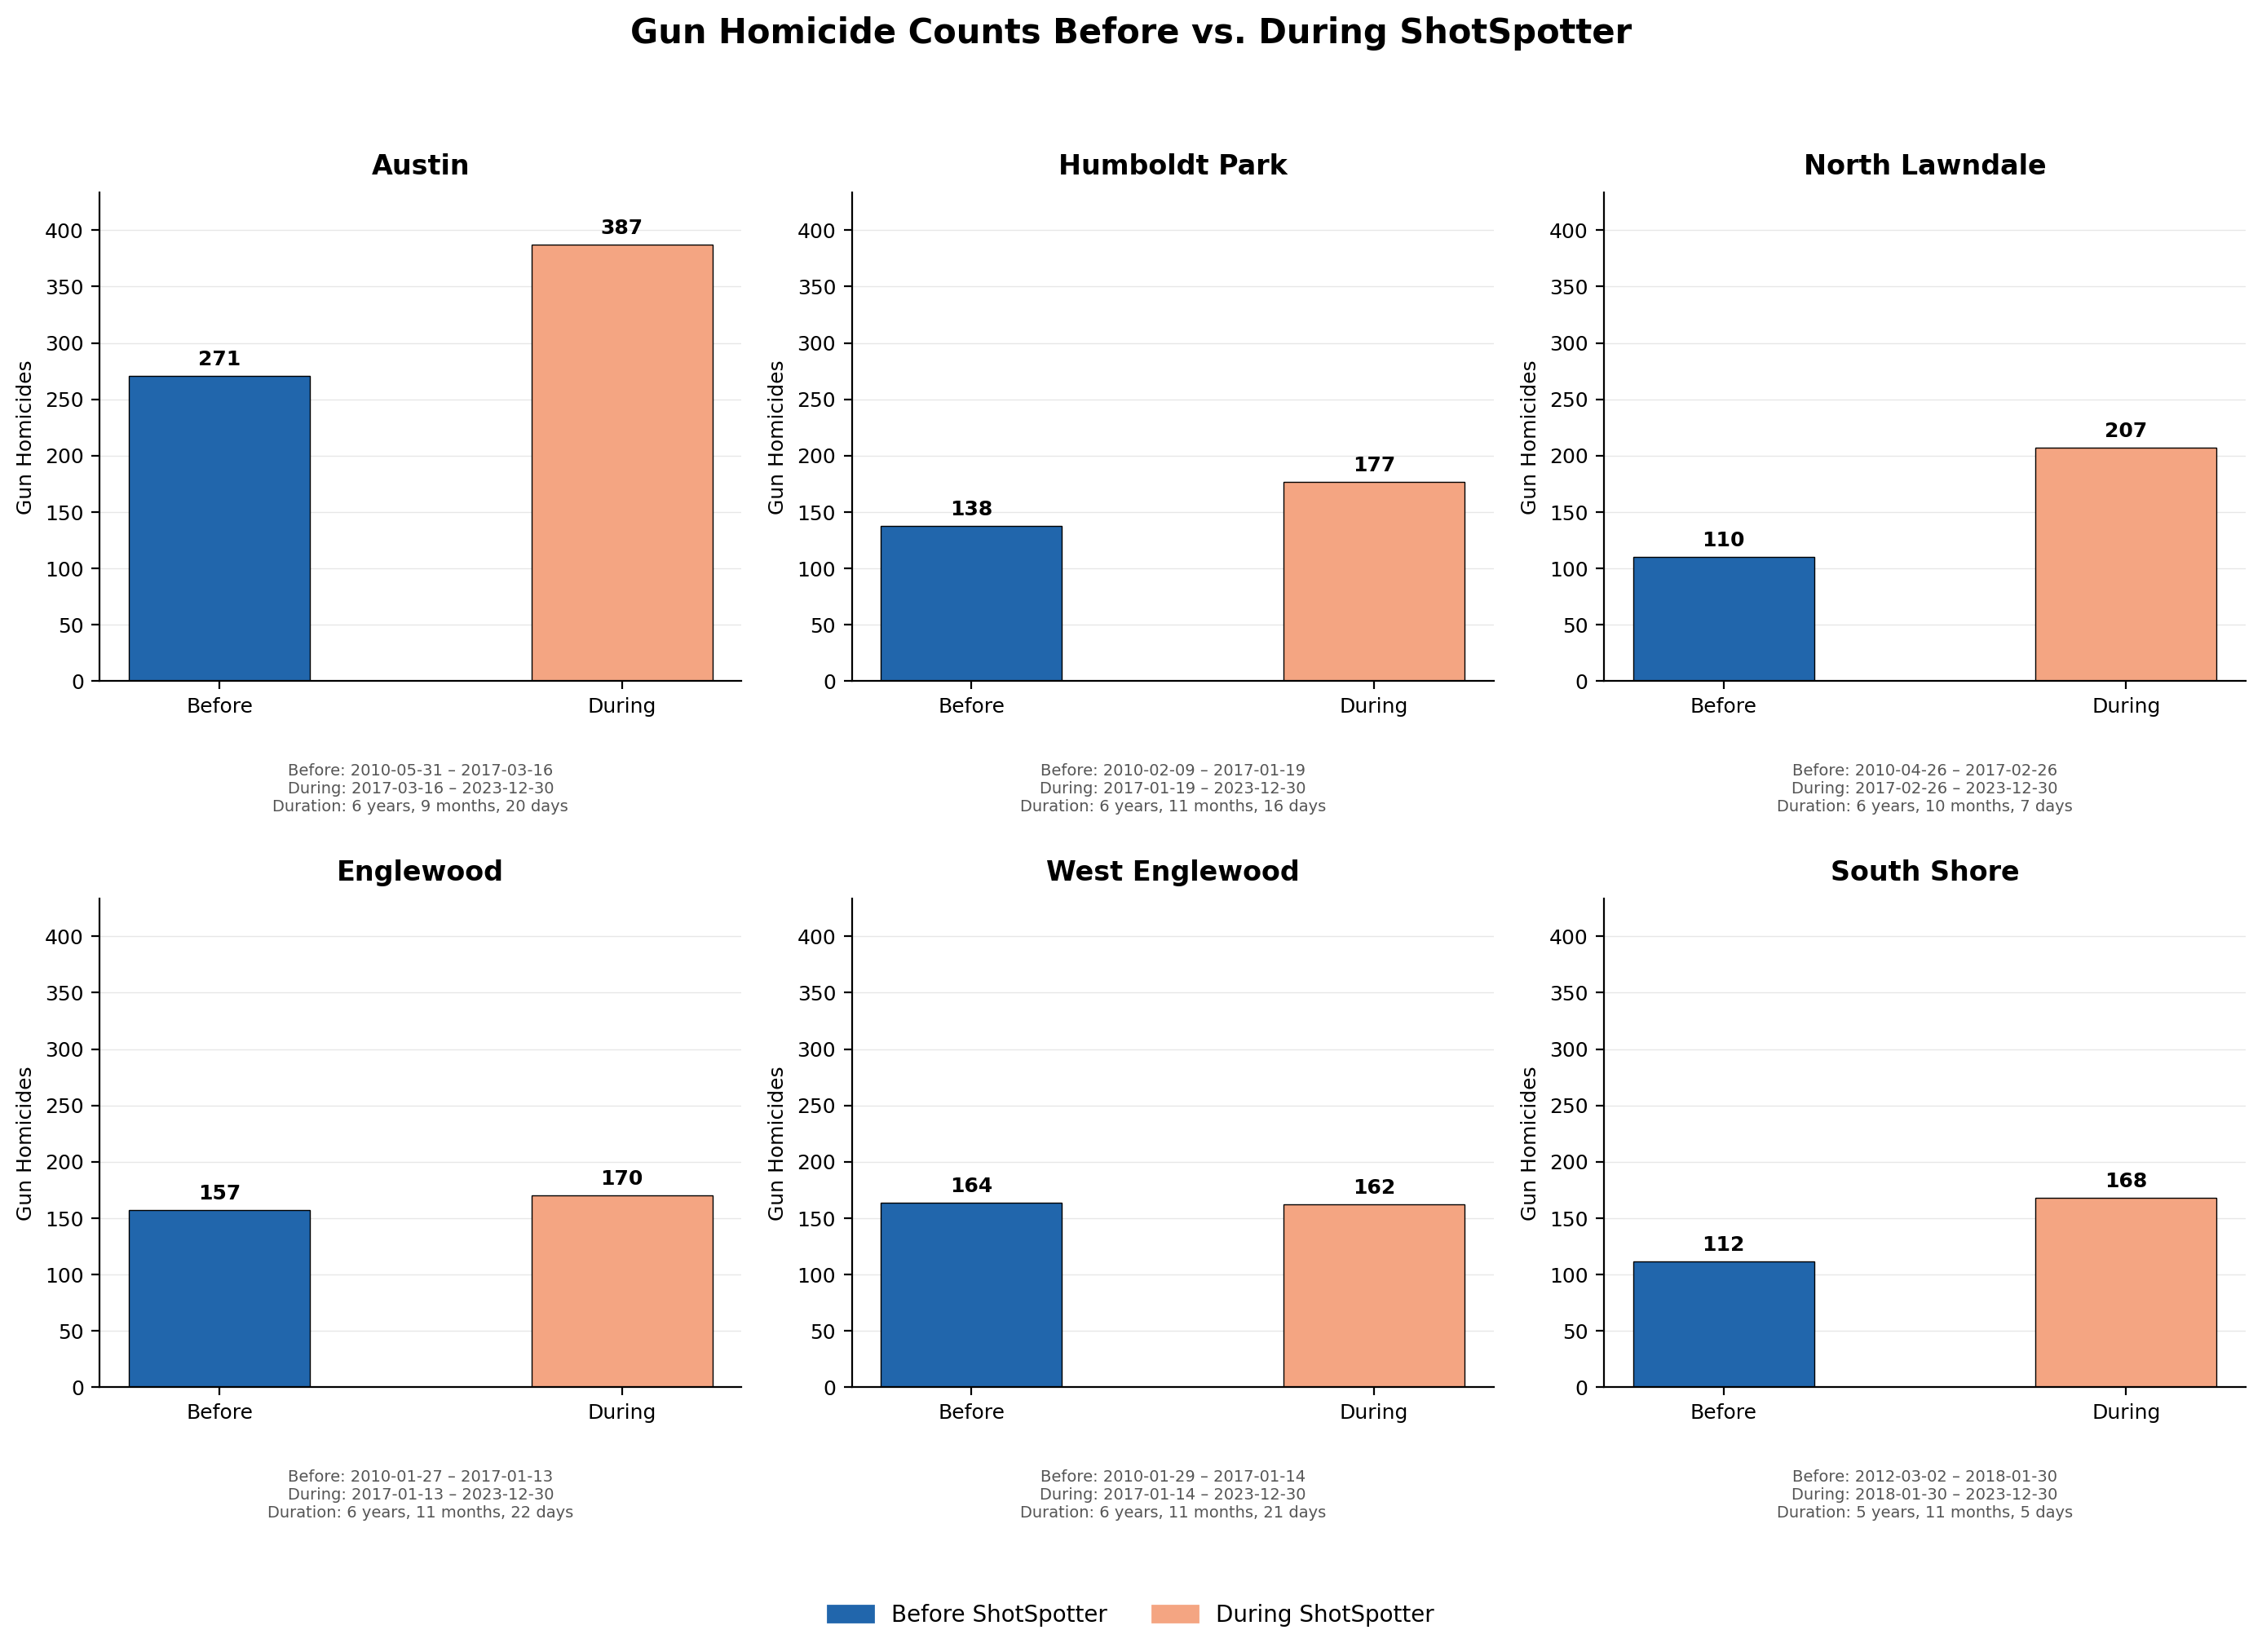
\includegraphics[width=0.95\textwidth]{homicide_comparison.png}
\caption{Total gun homicides before versus during ShotSpotter in each study
neighborhood. Raw counts rose in most neighborhoods, but this naive before/during
contrast confounds the intervention with the city-wide violence trend and with selection
into treatment.}
\label{fig:comparison}
\end{figure}

% ===========================================================================
\section{Empirical Strategy}

\subsection{The identification problem}

In a randomized experiment we would compare treated neighborhoods to a control group
drawn from the same distribution of pre-treatment violence. Chicago's data do not allow
that. Because the 51 ShotSpotter neighborhoods had roughly nine times the homicide rate
of the 26 non-ShotSpotter neighborhoods \emph{before} deployment, any
difference-in-differences contrast must lean on the parallel-trends assumption: that,
absent ShotSpotter, the two groups would have moved in parallel. Much of the paper is a
sustained test of whether that assumption can survive contact with the data.

\subsection{Specifications}

We estimate five classes of model.

\begin{enumerate}
\itemsep0.2em
\item \textbf{Two-way fixed-effects DiD.}
$\text{gun\_hom}_{it} = \beta\,(\text{treat}_i \times \text{post}_t) + \alpha_i +
\gamma_t + \varepsilon_{it}$, with cluster-robust standard errors at the community-area
level, estimated on the full panel and with three robustness restrictions (excluding
2016, excluding the COVID years 2020--2021, and excluding both).

\item \textbf{Count-data regression.} Poisson and Negative Binomial DiD with the same
two-way fixed effects, appropriate for integer homicide counts. The Negative Binomial
dispersion is \emph{estimated} (Cameron--Trivedi NB2 auxiliary regression; Cameron \&
Trivedi, 2013) rather than fixed at one.

\item \textbf{Event studies.} A transparent, hand-rolled cohort-specific ATT$(g,k)$
estimator (2017 and 2018 cohorts versus the 26 never-treated areas, sample-weighted,
bootstrap standard errors) and the modern \textbf{Callaway \& Sant'Anna (2021)}
group-time ATT (estimated with the \texttt{differences} package, influence-function
inference), which we treat as the authoritative staggered-rollout result.

\item \textbf{Synthetic control.} For each of the six study neighborhoods, weights over
the 26 never-treated areas are chosen to minimize pre-treatment squared error on annual
gun-homicide counts, subject to the simplex constraint (Abadie, Diamond, \& Hainmueller,
2010), with in-space permutation inference.

\item \textbf{Pre-period placebo / falsification.} The DiD is re-estimated with
treatment reassigned to fake years (1999, 2003, 2007, 2011) well before the actual
rollout. A non-null placebo coefficient flags spurious significance and undermines the
design.
\end{enumerate}

% ===========================================================================
\section{Results}

\subsection{ShotSpotter detected what it was designed to detect}

Alert volume in covered neighborhoods is enormous: roughly 222,000 alerts across about
seven years and 51 communities, with the heaviest-coverage areas (Austin, West
Englewood, Englewood, North Lawndale) generating 8,000--15,000 alerts each. Both alert
volume and homicide counts peak in the same months (May--August) and the same hours (10
PM to 1 AM); Figure~\ref{fig:hourly} shows the within-day co-movement. That co-movement is
expected---detected gunfire and gun homicide share the same late-night diurnal cycle---so we
read the figure only as validation that the sensor network captures the gunfire it was
purchased to capture, not as a finding in its own right. As a \emph{measurement
instrument}, ShotSpotter works. The question these data must answer is whether detection
translated into fewer homicides---and whether they can answer it at all.

\begin{figure}[H]
\centering
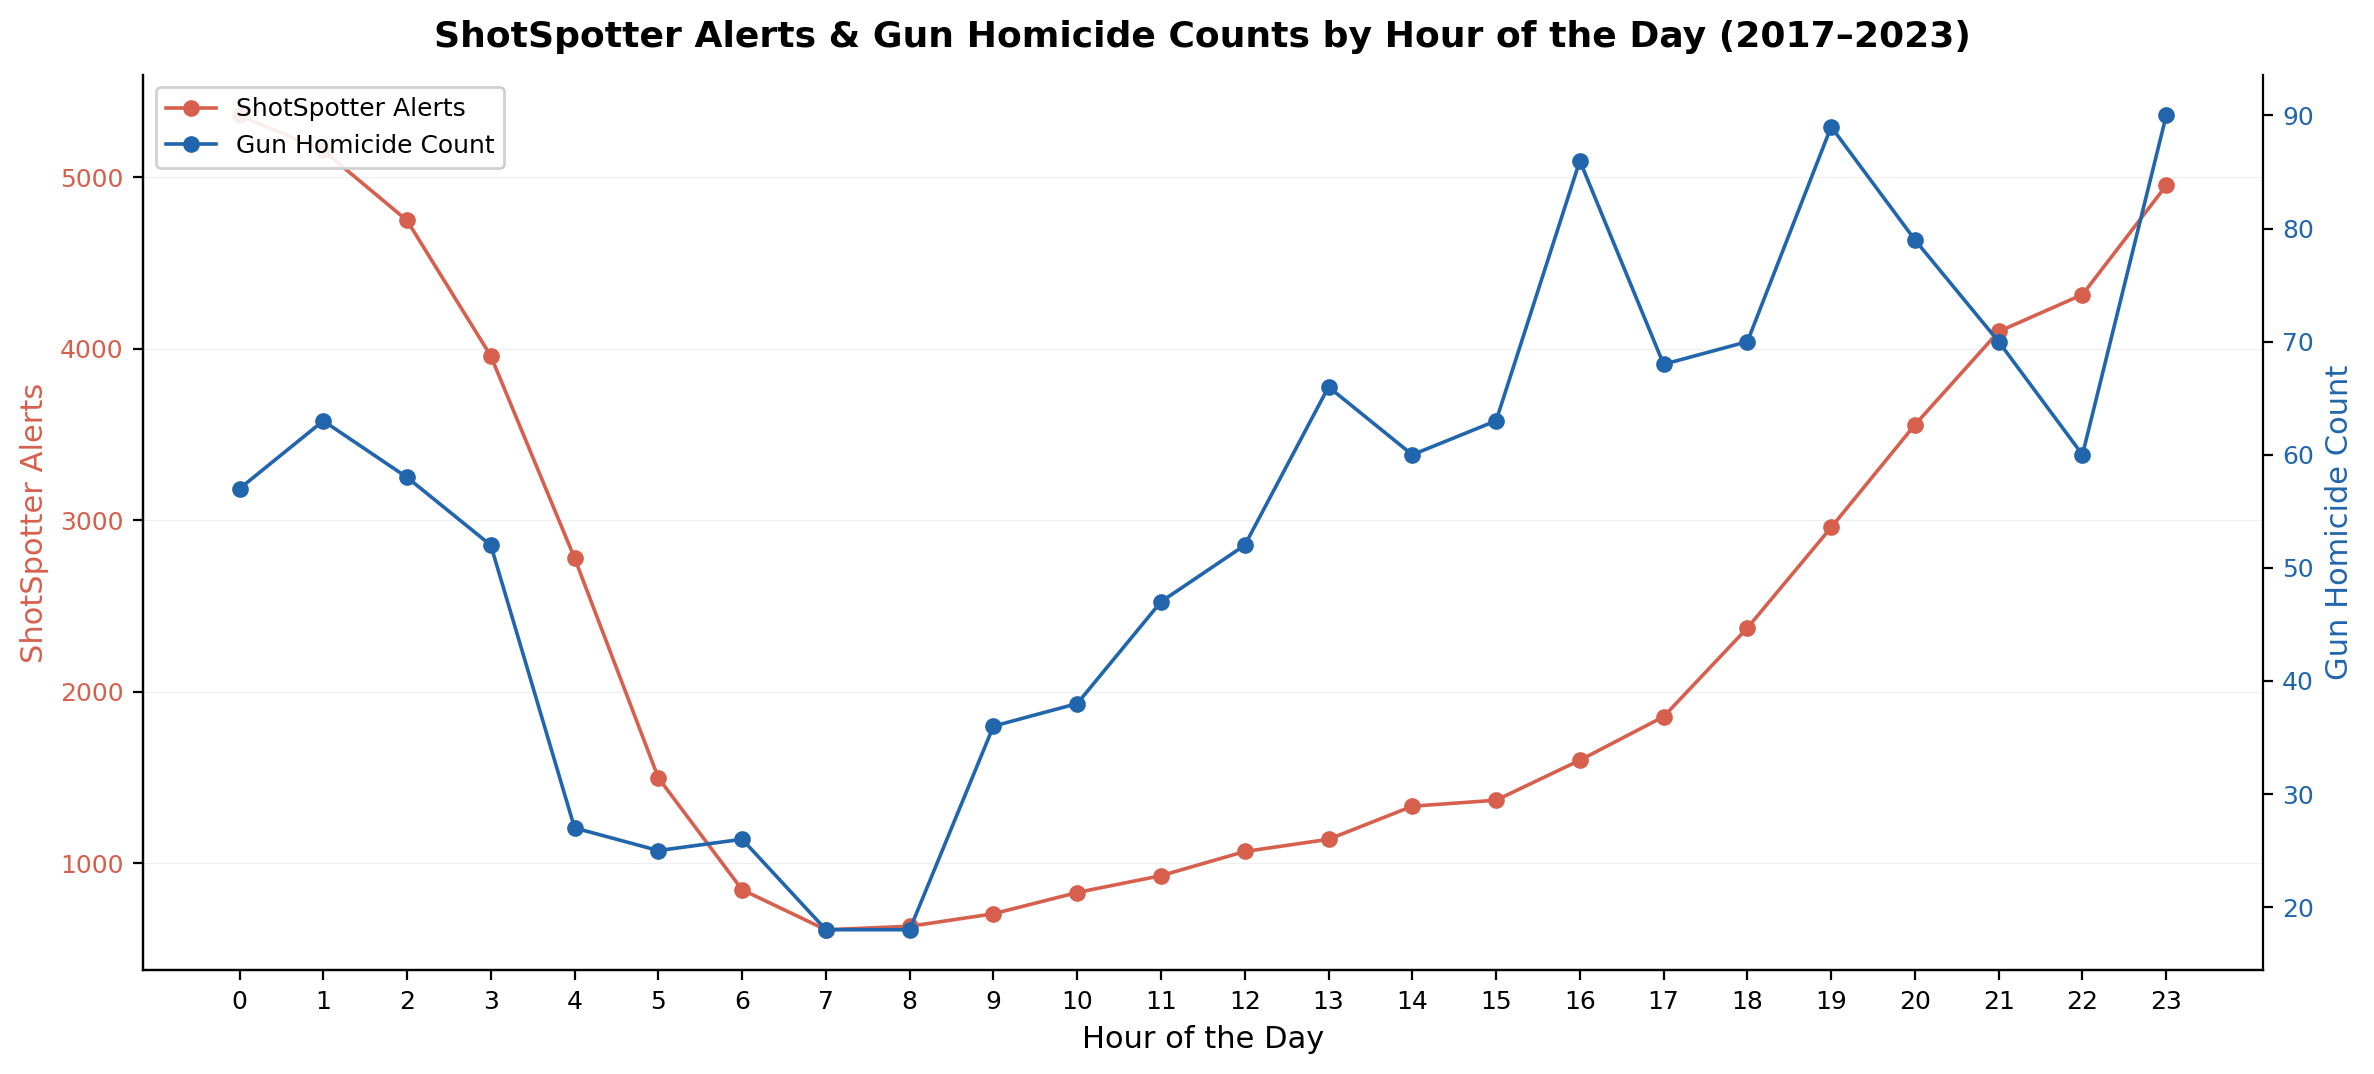
\includegraphics[width=0.9\textwidth]{hourly_pattern.png}
\caption{ShotSpotter alerts and gun homicides rise and fall together over the day, both
bottoming out mid-morning and peaking late at night---an expected co-movement, shown as
validation of the sensor network rather than as a finding. The system detects the gunfire
it is designed to detect.}
\label{fig:hourly}
\end{figure}

\subsection{The headline OLS DiD is positive---but disappears under count-data regression}

The two-way fixed-effects DiD coefficient on the full 2009--2023 panel is
$\beta = +2.627$ gun homicides per community-area-year (SE $= 0.638$, $p < 0.001$, 95\%
CI $[+1.38, +3.88]$). It is robust across restrictions: excluding COVID years yields
$+1.75$ ($p < 0.001$), excluding 2016 yields $+3.19$ ($p < 0.001$), and excluding both
yields $+2.31$ ($p < 0.001$) (Table~\ref{tab:twfe}). Crucially, the coefficient is
\emph{robust to fixed effects}---adding unit and year fixed effects reproduces the
original DiD coefficient almost exactly---so it does not come from a missing-controls
problem.

\begin{table}[H]
\centering
\small
\caption{Two-way fixed-effects OLS DiD on gun homicides (cluster-robust SEs).}
\label{tab:twfe}
\begin{tabular}{lccccc}
\toprule
Specification & $\beta$ (DiD) & SE & $p$ & 95\% CI & $N$ \\
\midrule
Full panel, 2009--2023        & $+2.627$ & 0.638 & $<0.001$ & $[+1.38, +3.88]$ & 1,155 \\
Excl.\ COVID (2020--21)       & $+1.749$ & 0.502 & $<0.001$ & $[+0.77, +2.73]$ & 1,001 \\
Excl.\ 2016                   & $+3.189$ & 0.767 & $<0.001$ & $[+1.69, +4.69]$ & 1,078 \\
Excl.\ COVID $+$ 2016         & $+2.311$ & 0.624 & $<0.001$ & $[+1.09, +3.54]$ & \phantom{0}924 \\
\bottomrule
\end{tabular}
\end{table}

What the headline is \emph{not} robust to is the choice of an appropriate model for count
data. Annual gun-homicide counts in a community area are small non-negative integers
whose variance grows with the mean; OLS treats them as continuous and homoscedastic,
weighting all observations equally and reporting an effect on the additive scale.
Poisson and Negative Binomial regressions let the variance scale with the mean and
estimate effects on the log scale, where they correspond to multiplicative (proportional)
changes---the natural metric for a percentage-effect treatment. Estimated this way, the
effect is \textbf{statistically null across every robustness specification}
(Table~\ref{tab:count}): Poisson and Negative Binomial incidence-rate ratios (IRRs)
hover around $1.07$ with confidence intervals consistent with anywhere from a 13\%
reduction to a 33\% increase in homicides. Because the estimated Negative Binomial
dispersion is small ($\alpha \approx 0.02$)---the counts are only mildly
overdispersed---the Negative Binomial IRRs land essentially on top of the Poisson
estimates. They also land essentially on top of the meta-analytic pooled effect for
gunshot detection (relative IRR $1.02$, 95\% CI $[0.90, 1.16]$; Huff, Dunlap, \& Pearson,
2026), estimated with the same incidence-rate-ratio metric---evidence that the
multiplicative-scale null is a property of the intervention, not an artifact of this
particular panel.

\begin{table}[H]
\centering
\small
\caption{Count-data DiD with two-way fixed effects. IRR $= \exp(\beta)$; an IRR of 1
means no effect.}
\label{tab:count}
\begin{tabular}{lcccc}
\toprule
Specification & $\beta$ & IRR & 95\% CI on IRR & $p$ \\
\midrule
OLS (TWFE), full panel                 & $+2.627$ & ---     & ---              & $<0.001$ \\
\midrule
Poisson (TWFE), full panel             & $+0.072$ & 1.074 & $[0.869, 1.328]$ & 0.508 \\
Poisson (TWFE), excl.\ COVID           & $+0.014$ & 1.014 & $[0.816, 1.259]$ & 0.902 \\
Poisson (TWFE), excl.\ 2016            & $+0.084$ & 1.087 & $[0.857, 1.381]$ & 0.491 \\
\midrule
Neg.\ Binomial, full panel             & $+0.067$ & 1.069 & $[0.860, 1.329]$ & 0.548 \\
Neg.\ Binomial, excl.\ COVID           & $+0.014$ & 1.014 & $[0.810, 1.269]$ & 0.902 \\
Neg.\ Binomial, excl.\ 2016            & $+0.074$ & 1.077 & $[0.844, 1.373]$ & 0.551 \\
\bottomrule
\end{tabular}
\end{table}

Figure~\ref{fig:spec} shows the contrast in one picture: the OLS effect, placed on the
multiplicative scale for comparison (implied IRR $\approx 1.35$, $p < 0.001$), against the
genuinely estimated Poisson and Negative Binomial IRRs, both of which collapse the
headline to a null near 1.07. Whatever the OLS DiD is picking up, it is being amplified
by the additive scale and by the unequal variance across community areas; on the natural
multiplicative scale, no effect is detectable. Figure~\ref{fig:forest} shows the same
heterogeneity at the neighborhood level: individual before/after changes in the
gun-homicide rate range from about $-2\%$ (West Englewood) to $+62\%$ (South Shore), and
even the pooled estimate ($+23\%$, excluding COVID) carries a wide interval.
For completeness, non-fatal gunshot injuries (a four-times-larger sample) yield $\beta =
+7.51$ under OLS ($p = 0.009$)---and the count-data correction is even starker there:
estimated as Poisson or Negative Binomial with the same fixed effects, the point estimate
flips \emph{below} one and is statistically null in every specification (IRRs
$0.84$--$0.92$, $p \geq 0.23$). The higher-powered outcome delivers the same verdict as
the homicide series: the additive OLS coefficient is a scale artifact.

\begin{figure}[H]
\centering
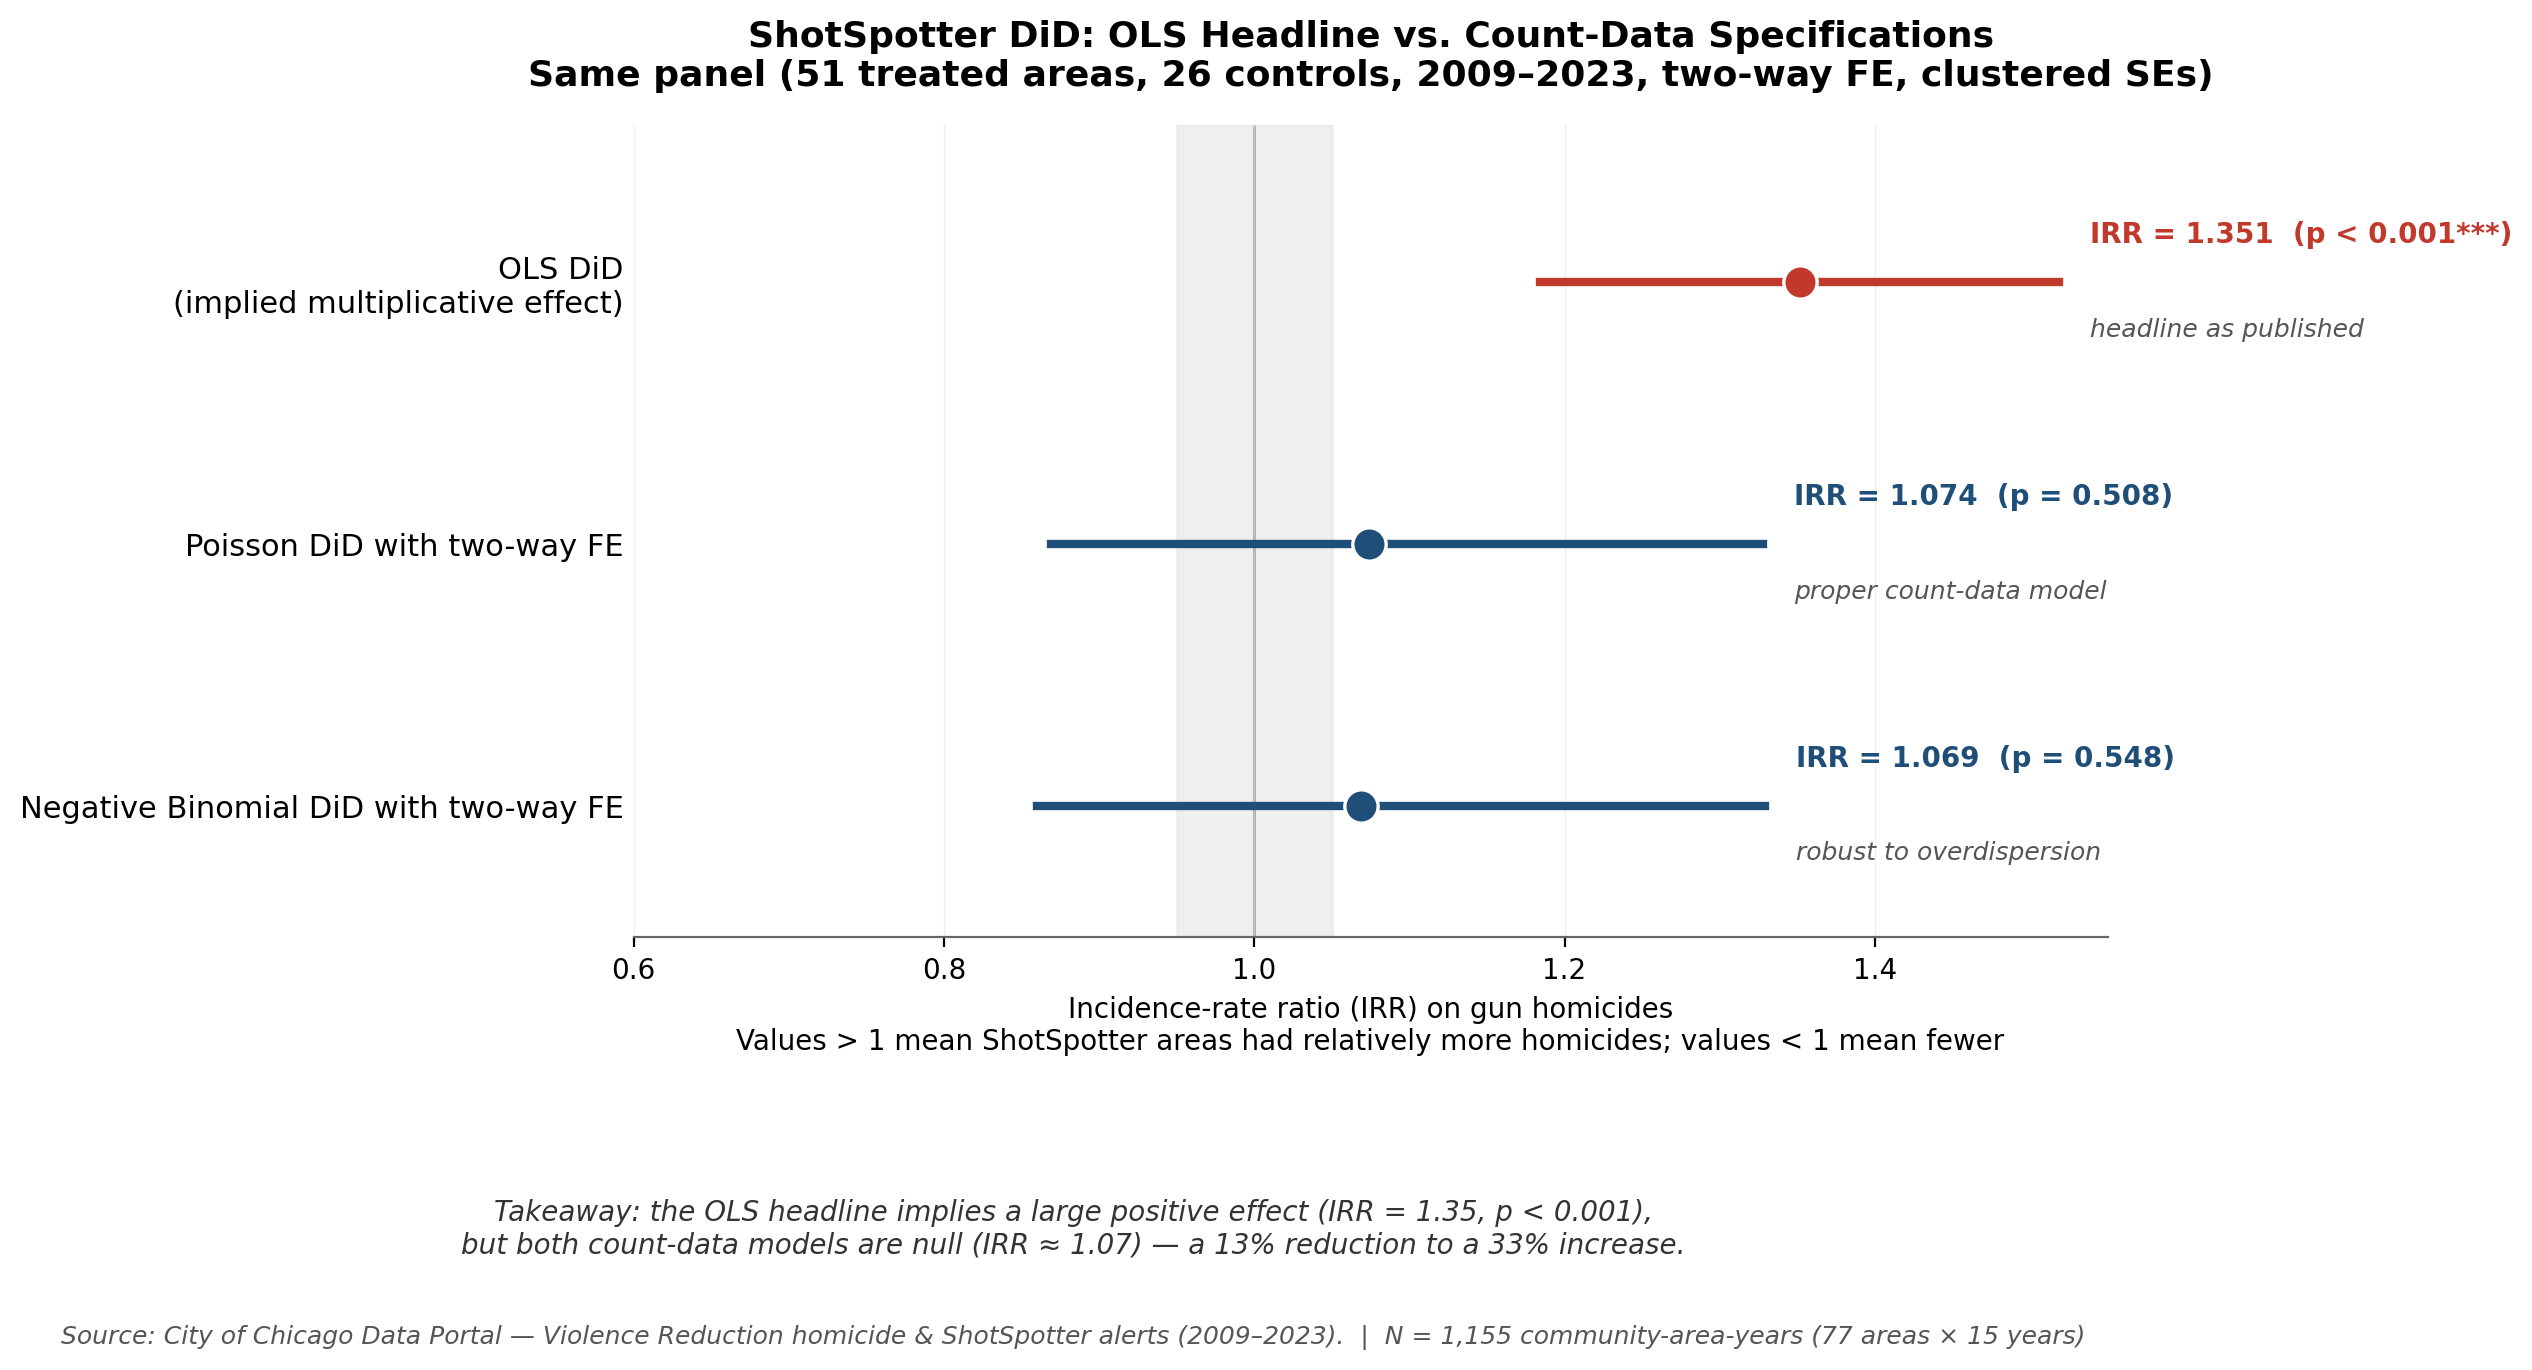
\includegraphics[width=0.85\textwidth]{specification_comparison.png}
\caption{The whole story in one figure. The OLS effect is the additive $+2.63$
coefficient shown on the multiplicative scale for comparison (implied IRR $\approx 1.35$,
$p < 0.001$); the Poisson and Negative Binomial points are genuinely estimated
incidence-rate ratios. Both count-data models collapse the headline to a statistically
null IRR $\approx 1.07$.}
\label{fig:spec}
\end{figure}

\begin{figure}[H]
\centering
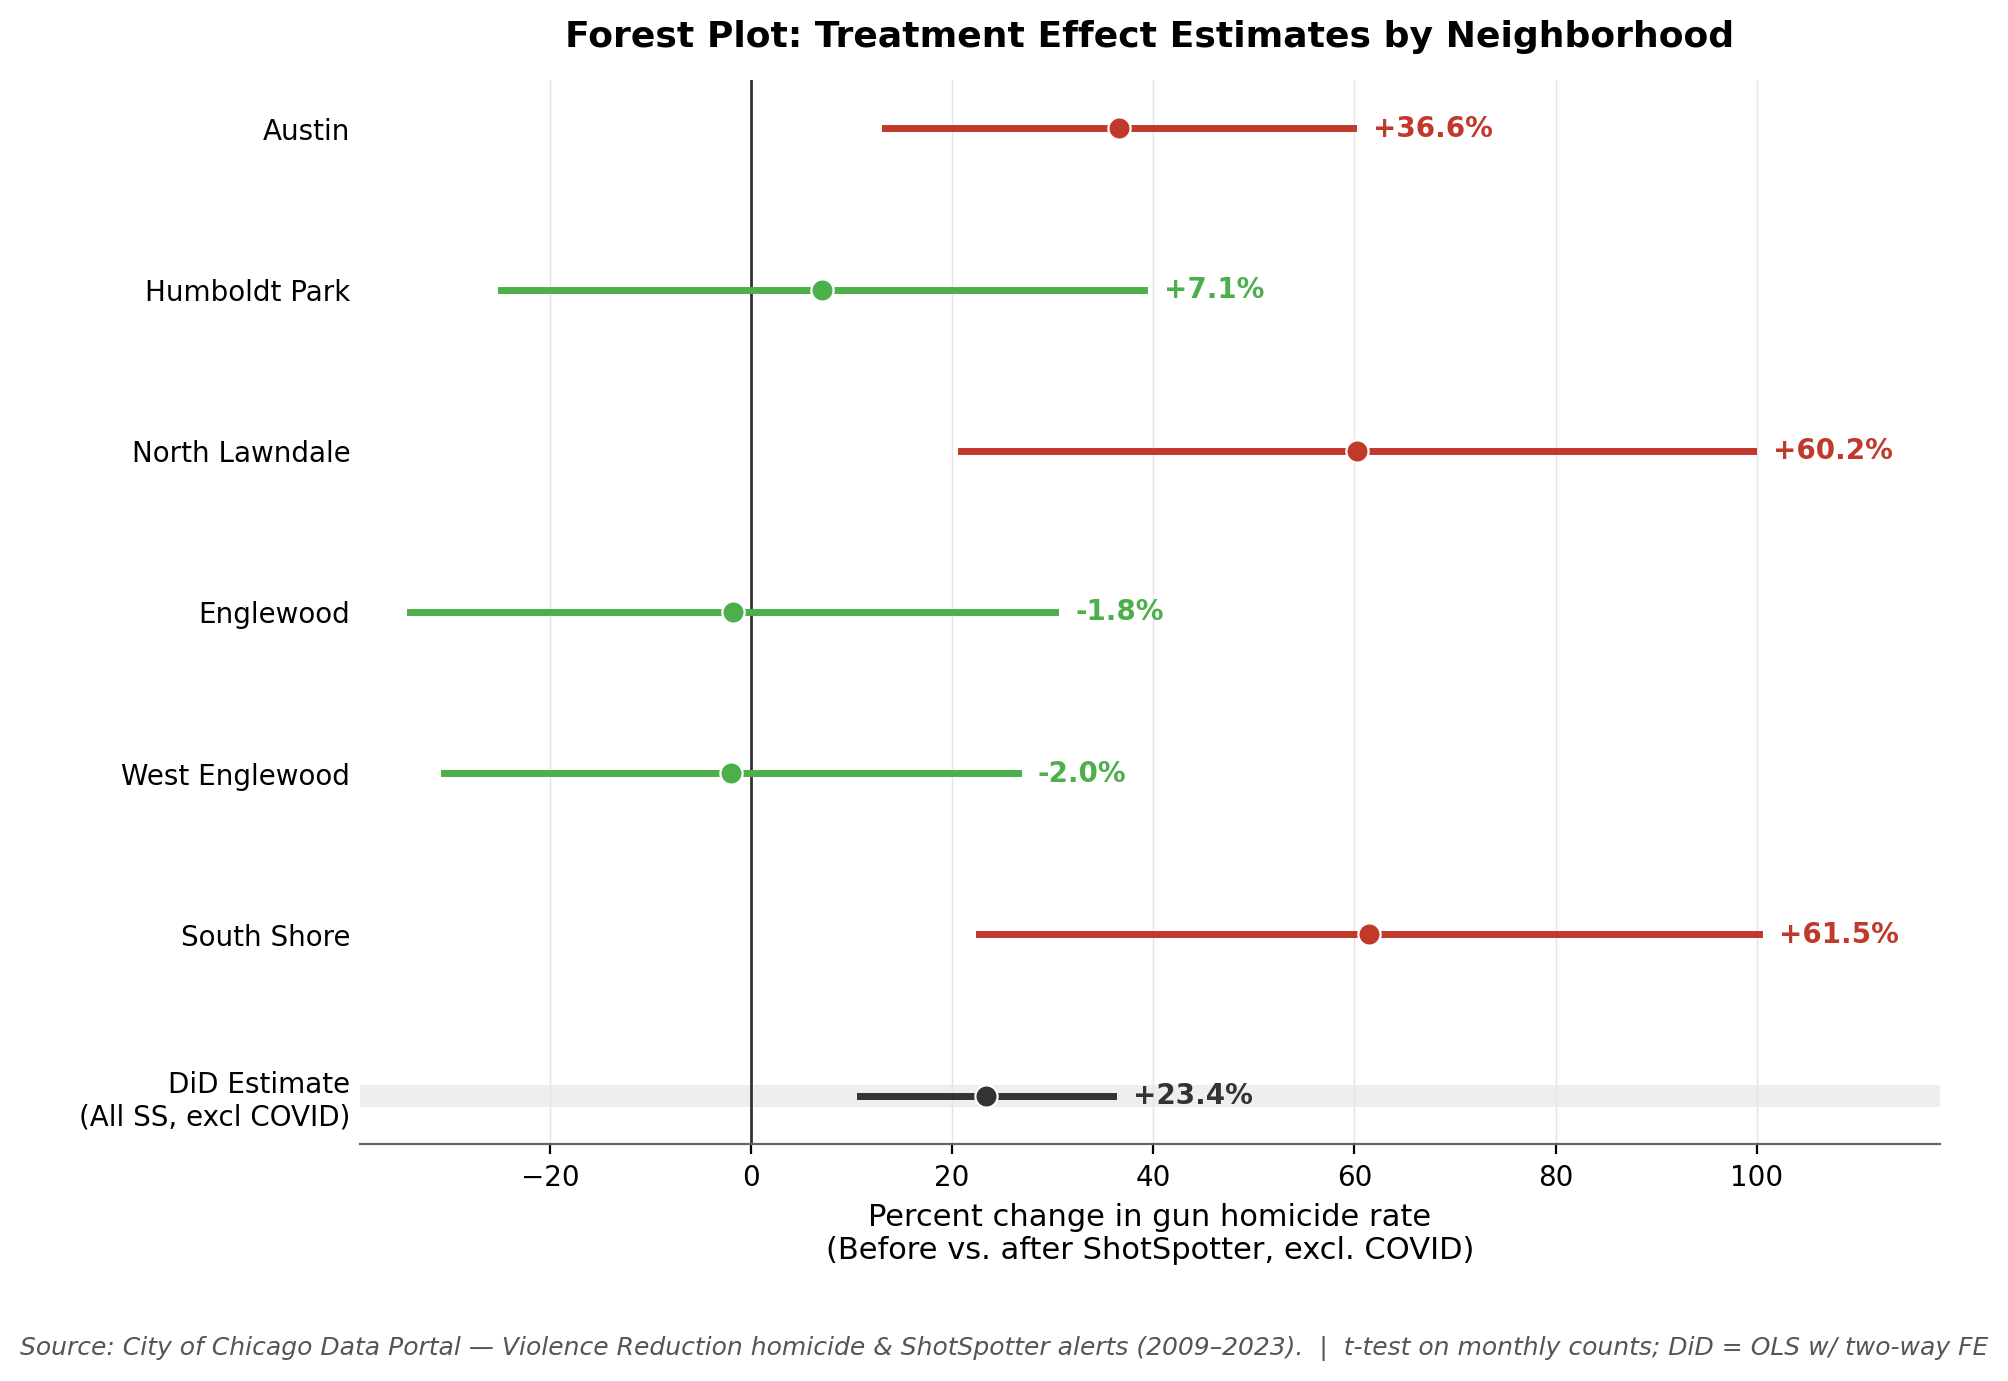
\includegraphics[width=0.82\textwidth]{forest_plot_effects.png}
\caption{Neighborhood-level before/after change in the gun-homicide rate (excluding
COVID), with the pooled DiD estimate at the bottom; changes whose intervals exclude zero
in red, others in gray. The spread across neighborhoods---from roughly $-2\%$ to
$+62\%$---shows how heavily the pooled headline leans on a few high-count neighborhoods.}
\label{fig:forest}
\end{figure}

\subsection{The design produces ``significant'' placebos}

If the $+2.627$ reflected a real treatment effect, then assigning \emph{fake} treatment
dates well before the actual rollout should yield null estimates. It does not
(Table~\ref{tab:placebo}). Two of four placebos are statistically significant at the 1\%
level, with magnitudes (1.3--1.9 homicides per area-year) on the same order as the
post-2017 estimate. They are opposite-signed, but that is precisely the point: a design
that manufactures ``significant'' effects in years before the program existed is
capturing pre-existing trend differences across neighborhoods---most likely the
long-run, differentially absorbed city-wide decline from the early-1990s
peak---not the intervention. That a difference-in-differences specification can return
spurious significance is exactly the pathology Bertrand, Duflo, and Mullainathan (2004)
documented, in which conventional standard errors so understate uncertainty that a large
share of randomly dated placebo interventions test as significant. Figure~\ref{fig:falsification} plots the placebo
coefficients against the true post-2017 estimate.

\begin{table}[H]
\centering
\small
\caption{Pre-period placebo tests: DiD with treatment reassigned to fake pre-rollout years.}
\label{tab:placebo}
\begin{tabular}{lcccc}
\toprule
Fake treatment year & $\beta$ & SE & $p$ & 95\% CI \\
\midrule
1999 & $-1.344$ & 0.507 & 0.008 & $[-2.34, -0.35]$ \\
2003 & $-1.929$ & 0.714 & 0.007 & $[-3.33, -0.53]$ \\
2007 & $-0.645$ & 0.497 & 0.194 & $[-1.62, +0.33]$ \\
2011 & $+0.256$ & 0.347 & 0.461 & $[-0.42, +0.94]$ \\
\bottomrule
\end{tabular}
\end{table}

\begin{figure}[H]
\centering
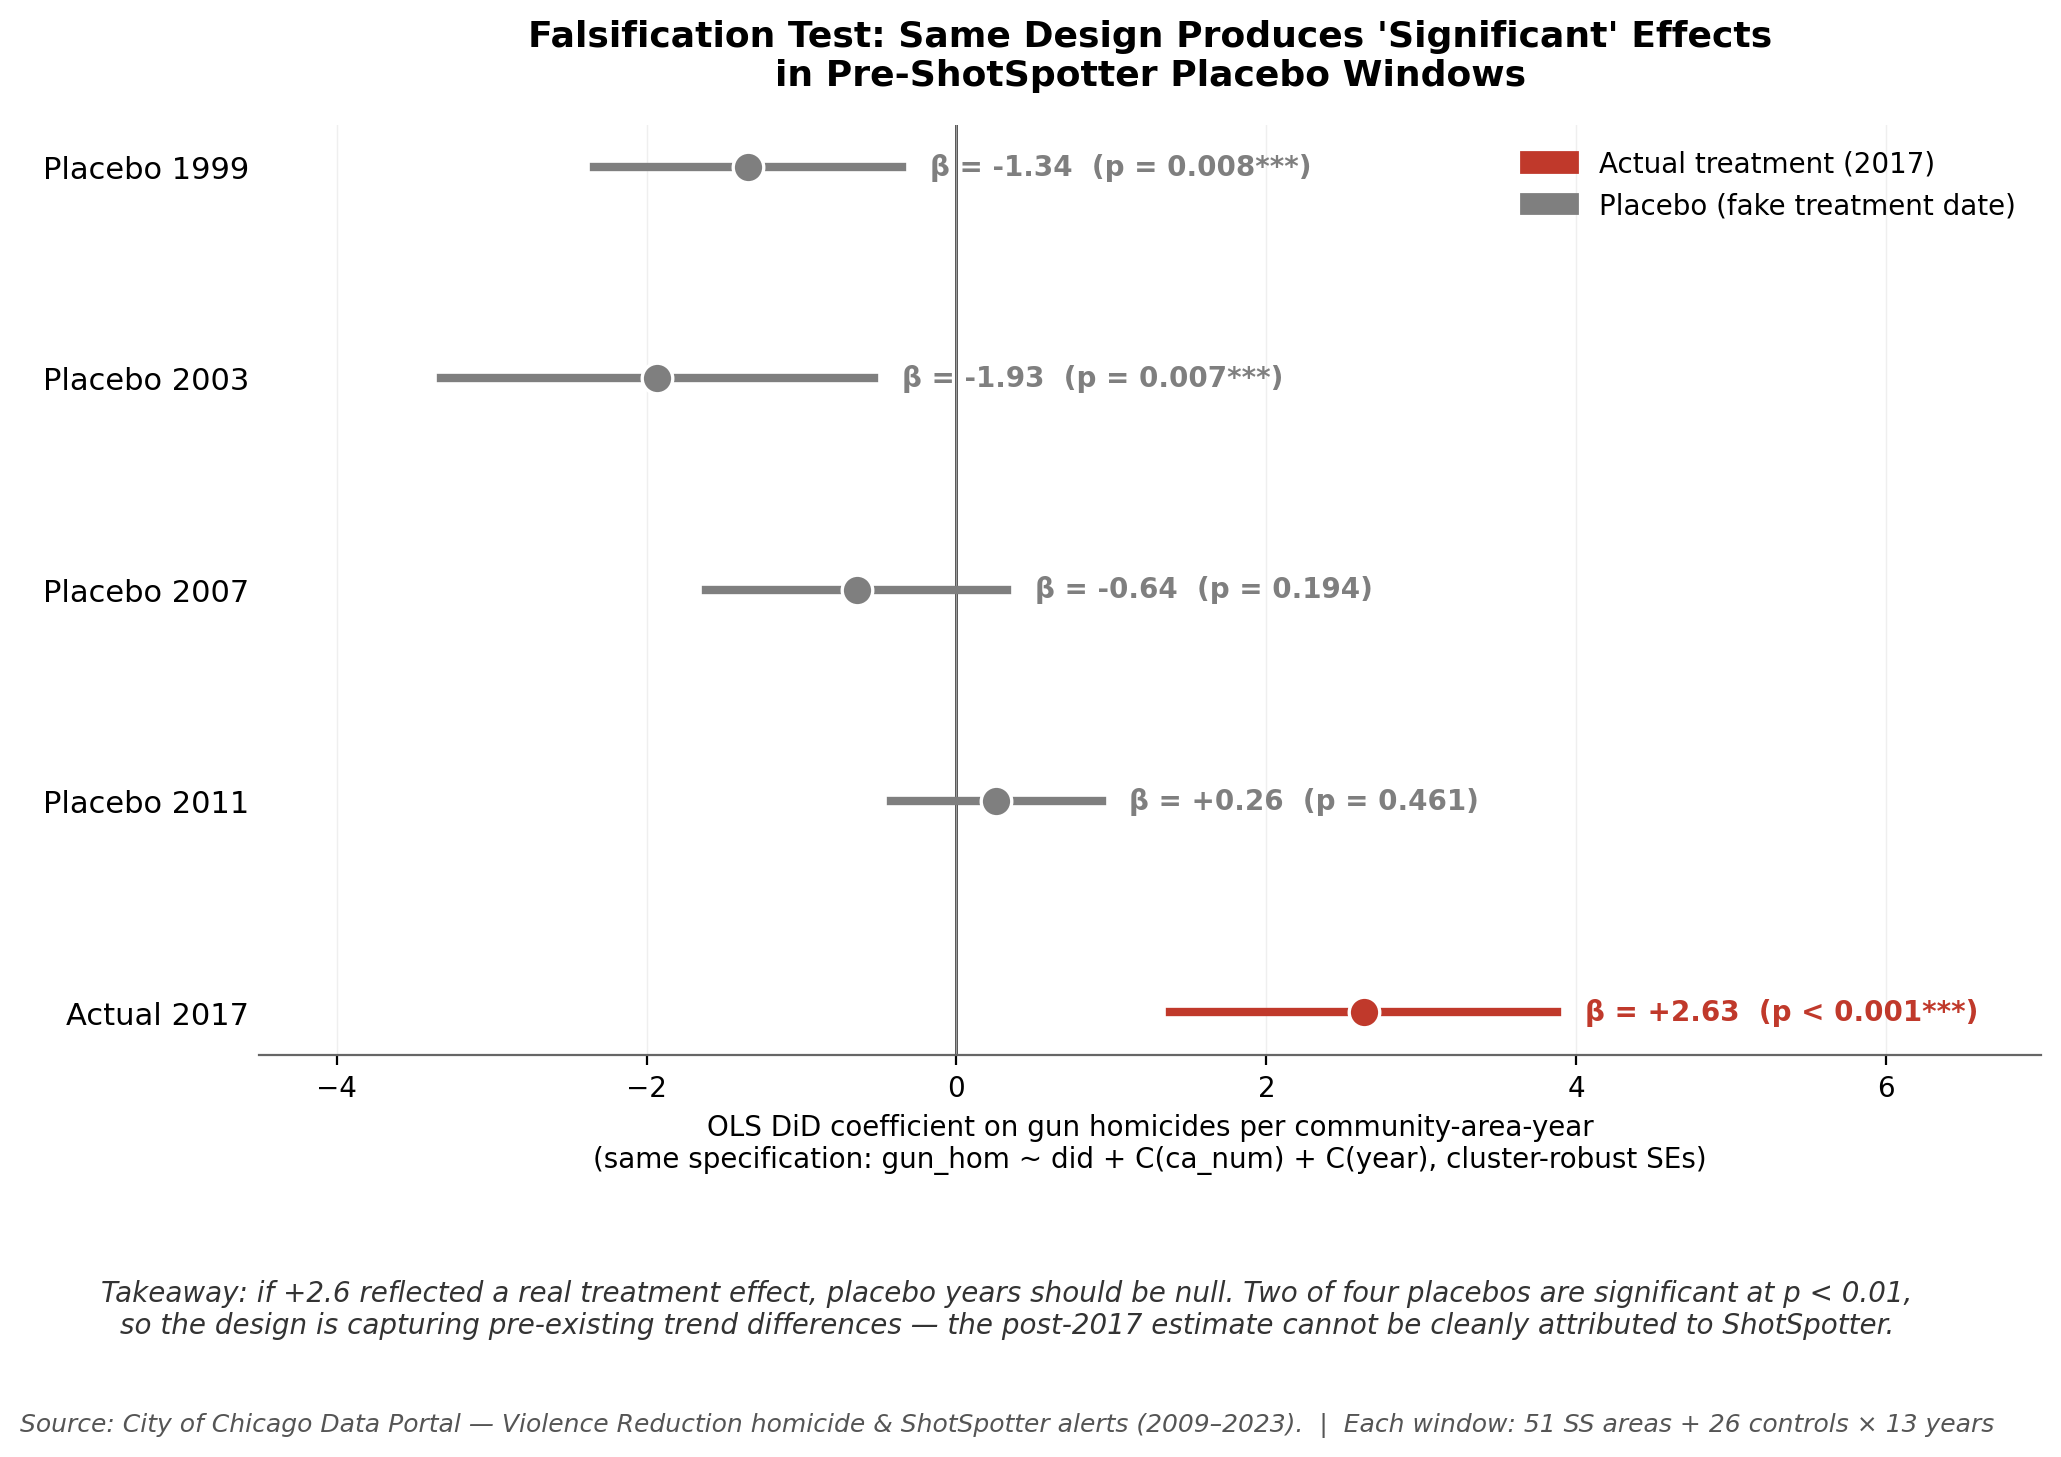
\includegraphics[width=0.85\textwidth]{falsification_plot.png}
\caption{Falsification test. Assigning fake treatment dates before ShotSpotter existed
should produce null effects; instead the 1999 and 2003 placebos come back significant at
the 1\% level and of comparable magnitude to the true post-2017 estimate.}
\label{fig:falsification}
\end{figure}

\subsection{The event studies confirm a failure of parallel trends}

The cohort-specific event study (Table~\ref{tab:eventstudy}, aggregated across the 2017
and 2018 cohorts with never-treated controls) shows that \emph{every} pre-treatment
coefficient is large and negative---a clear failure of parallel trends. A formal joint
Wald $F$-test on the seven pre-treatment interaction coefficients, which is invariant to
the choice of base year, yields $F = 19.9$, $p = 0.006$, rejecting parallel trends at the
1\% level. The pattern is mechanical: 2016 was a Chicago-wide homicide-record year,
disproportionately concentrated in the neighborhoods that would soon receive ShotSpotter,
and the event study uses a year adjacent to 2016 as its base, so every other year looks
anomalously low (Figure~\ref{fig:eventstudy}). Once a design fails this test, the DiD
contrast cannot be read as causal. This is not a technicality to be tested away: pre-trends
tests are themselves underpowered, and conditioning on having ``passed'' one distorts the
inference that follows (Roth, 2022). A design that visibly \emph{fails} the test, as this
one does, is telling us the parallel-trends assumption is not available---and the credible
response is to report that the effect is not point-identified, not to lean on a single
base-year normalization.

\begin{table}[H]
\centering
\small
\caption{Cohort-specific event study, aggregated ATT by event time $k$ (years from
install), sample-weighted, bootstrap CIs.}
\label{tab:eventstudy}
\begin{tabular}{ccc}
\toprule
$k$ (years from install) & ATT & 95\% CI \\
\midrule
$-7$ & $-5.46$ & $[-9.30, -1.62]$ \\
$-6$ & $-4.54$ & $[-8.53, -0.56]$ \\
$-5$ & $-5.09$ & $[-8.97, -1.20]$ \\
$-4$ & $-6.25$ & $[-10.04, -2.46]$ \\
$-3$ & $-6.09$ & $[-10.01, -2.17]$ \\
$-2$ & $-4.92$ & $[-8.92, -0.93]$ \\
$-1$ (base) & $0$ & --- \\
$\phantom{+}0$ & $-1.95$ & $[-6.57, +2.68]$ \\
$+1$ & $-4.65$ & $[-8.79, -0.51]$ \\
$+2$ & $-3.83$ & $[-8.12, +0.47]$ \\
$+3$ & $+0.10$ & $[-4.85, +5.05]$ \\
$+4$ & $-0.43$ & $[-5.25, +4.39]$ \\
$+5$ & $-2.99$ & $[-7.19, +1.22]$ \\
\bottomrule
\end{tabular}
\end{table}

\begin{figure}[H]
\centering
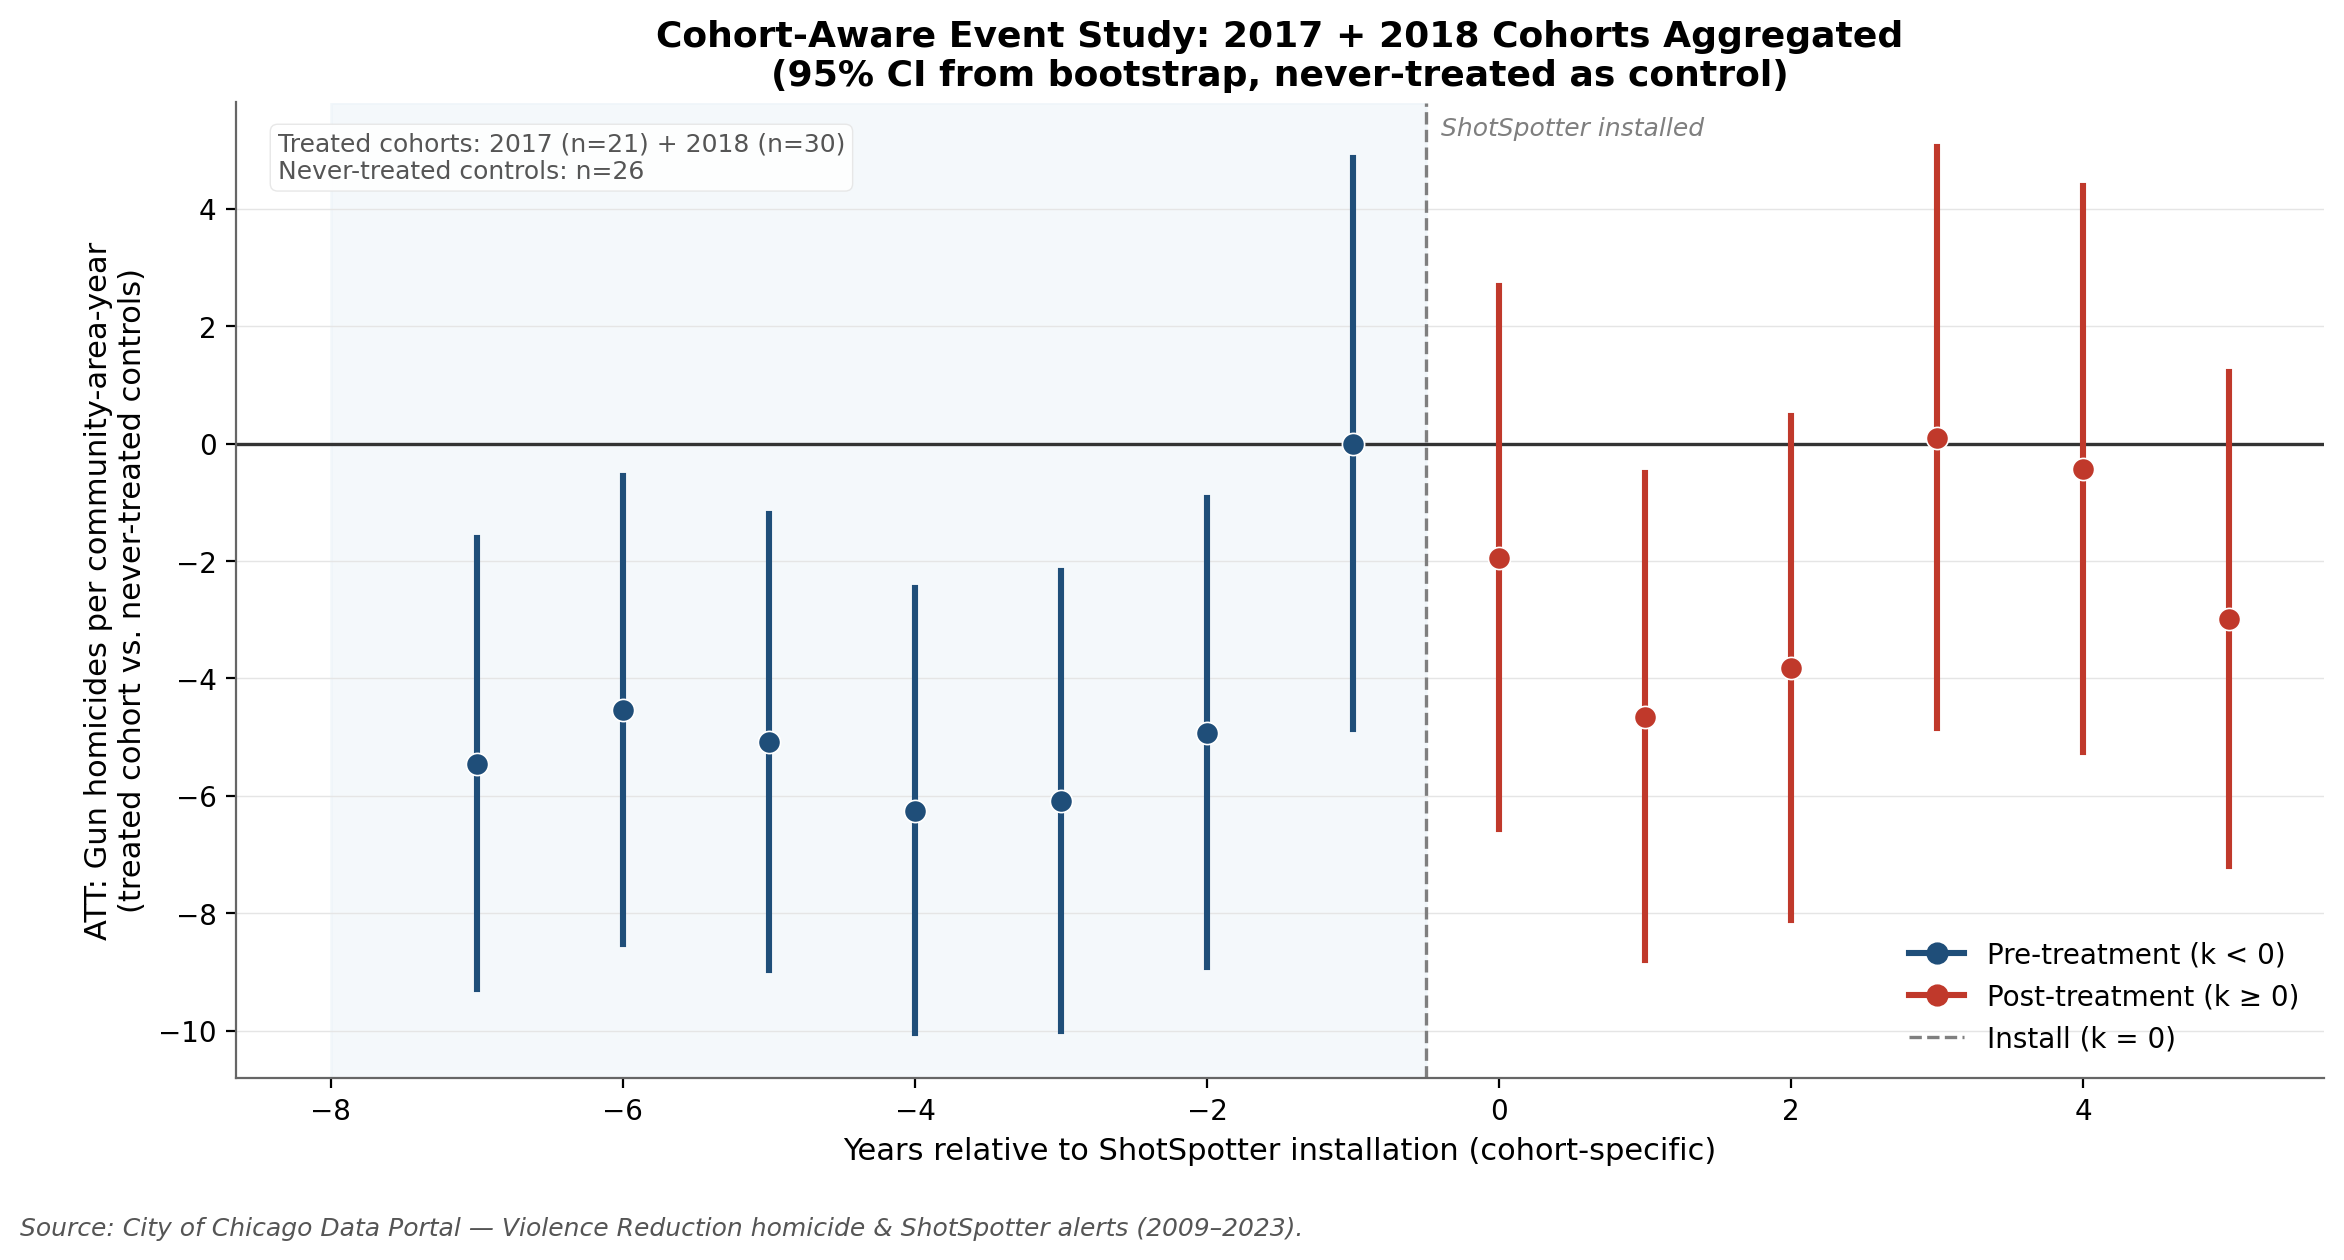
\includegraphics[width=0.85\textwidth]{event_study_cohort_aware.png}
\caption{Cohort-aware event study with bootstrap confidence intervals. Large negative
pre-treatment coefficients reveal a violation of parallel trends driven by the 2016
record-homicide year sitting next to the base period.}
\label{fig:eventstudy}
\end{figure}

The hand-rolled event study is intuitive but is not the modern estimator the
staggered-rollout literature prescribes. As a final check we re-estimate the effect with
the \textbf{Callaway \& Sant'Anna (2021)} group-time ATT
(Table~\ref{tab:cs}). On the full panel the overall ATT is $-2.45$ per
community-area-year (SE $0.89$)---\emph{negative}, the opposite sign of the pooled OLS,
and stable to using not-yet-treated rather than never-treated controls ($-2.51$). But
this negative sign is not a property of the estimator. It is driven almost entirely by
the 2016 record-homicide year, which sits at the $k = -1$ baseline for the 2017 cohort:
the event study shows that only the $k = -1$ (2016) pre-coefficient is significant while
the rest hover at zero, and \textbf{excluding 2016 and re-estimating returns $+1.90$ (SE
$0.72$)---the same sign as the OLS DiD} (Figure~\ref{fig:cs}). The apparent
OLS-versus-Callaway--Sant'Anna sign reversal is therefore a single-year sensitivity, not
a sign that the estimators fundamentally disagree about a well-identified parameter. The
Callaway--Sant'Anna estimator is precisely the tool the staggered-adoption literature
prescribes to remove the negative weighting that can flip a two-way fixed-effects
coefficient under heterogeneous timing (Goodman-Bacon, 2021; de Chaisemartin \&
D'Haultf\oe uille, 2020). That even it returns a sign contingent on a single year confirms
the parameter is not identified in these data, rather than restoring it. A
Goodman--Bacon decomposition of the staggered two-way fixed-effects estimate ($+2.48$,
cohort-specific timing) locates the problem precisely: the ``forbidden'' comparison of
the 2018 cohort against the already-treated 2017 cohort carries only $4.6\%$ of the
weight, and the weighted 2$\times$2 components reproduce the aggregate exactly
(Figure~\ref{fig:bacon}). Negative-weighting contamination is therefore minor in this
panel---the instability comes from the 2016 anomaly and the absence of a valid control
group, not from the staggered aggregation itself.

\begin{table}[H]
\centering
\small
\caption{Callaway--Sant'Anna (2021) overall ATT, gun homicides per community-area-year.}
\label{tab:cs}
\begin{tabular}{lcc}
\toprule
Control group & Overall ATT & SE \\
\midrule
Never-treated                 & $-2.453$ & 0.893 \\
Not-yet-treated               & $-2.508$ & 0.898 \\
Never-treated, excl.\ 2016    & $+1.895$ & 0.724 \\
\bottomrule
\end{tabular}
\end{table}

\begin{figure}[H]
\centering
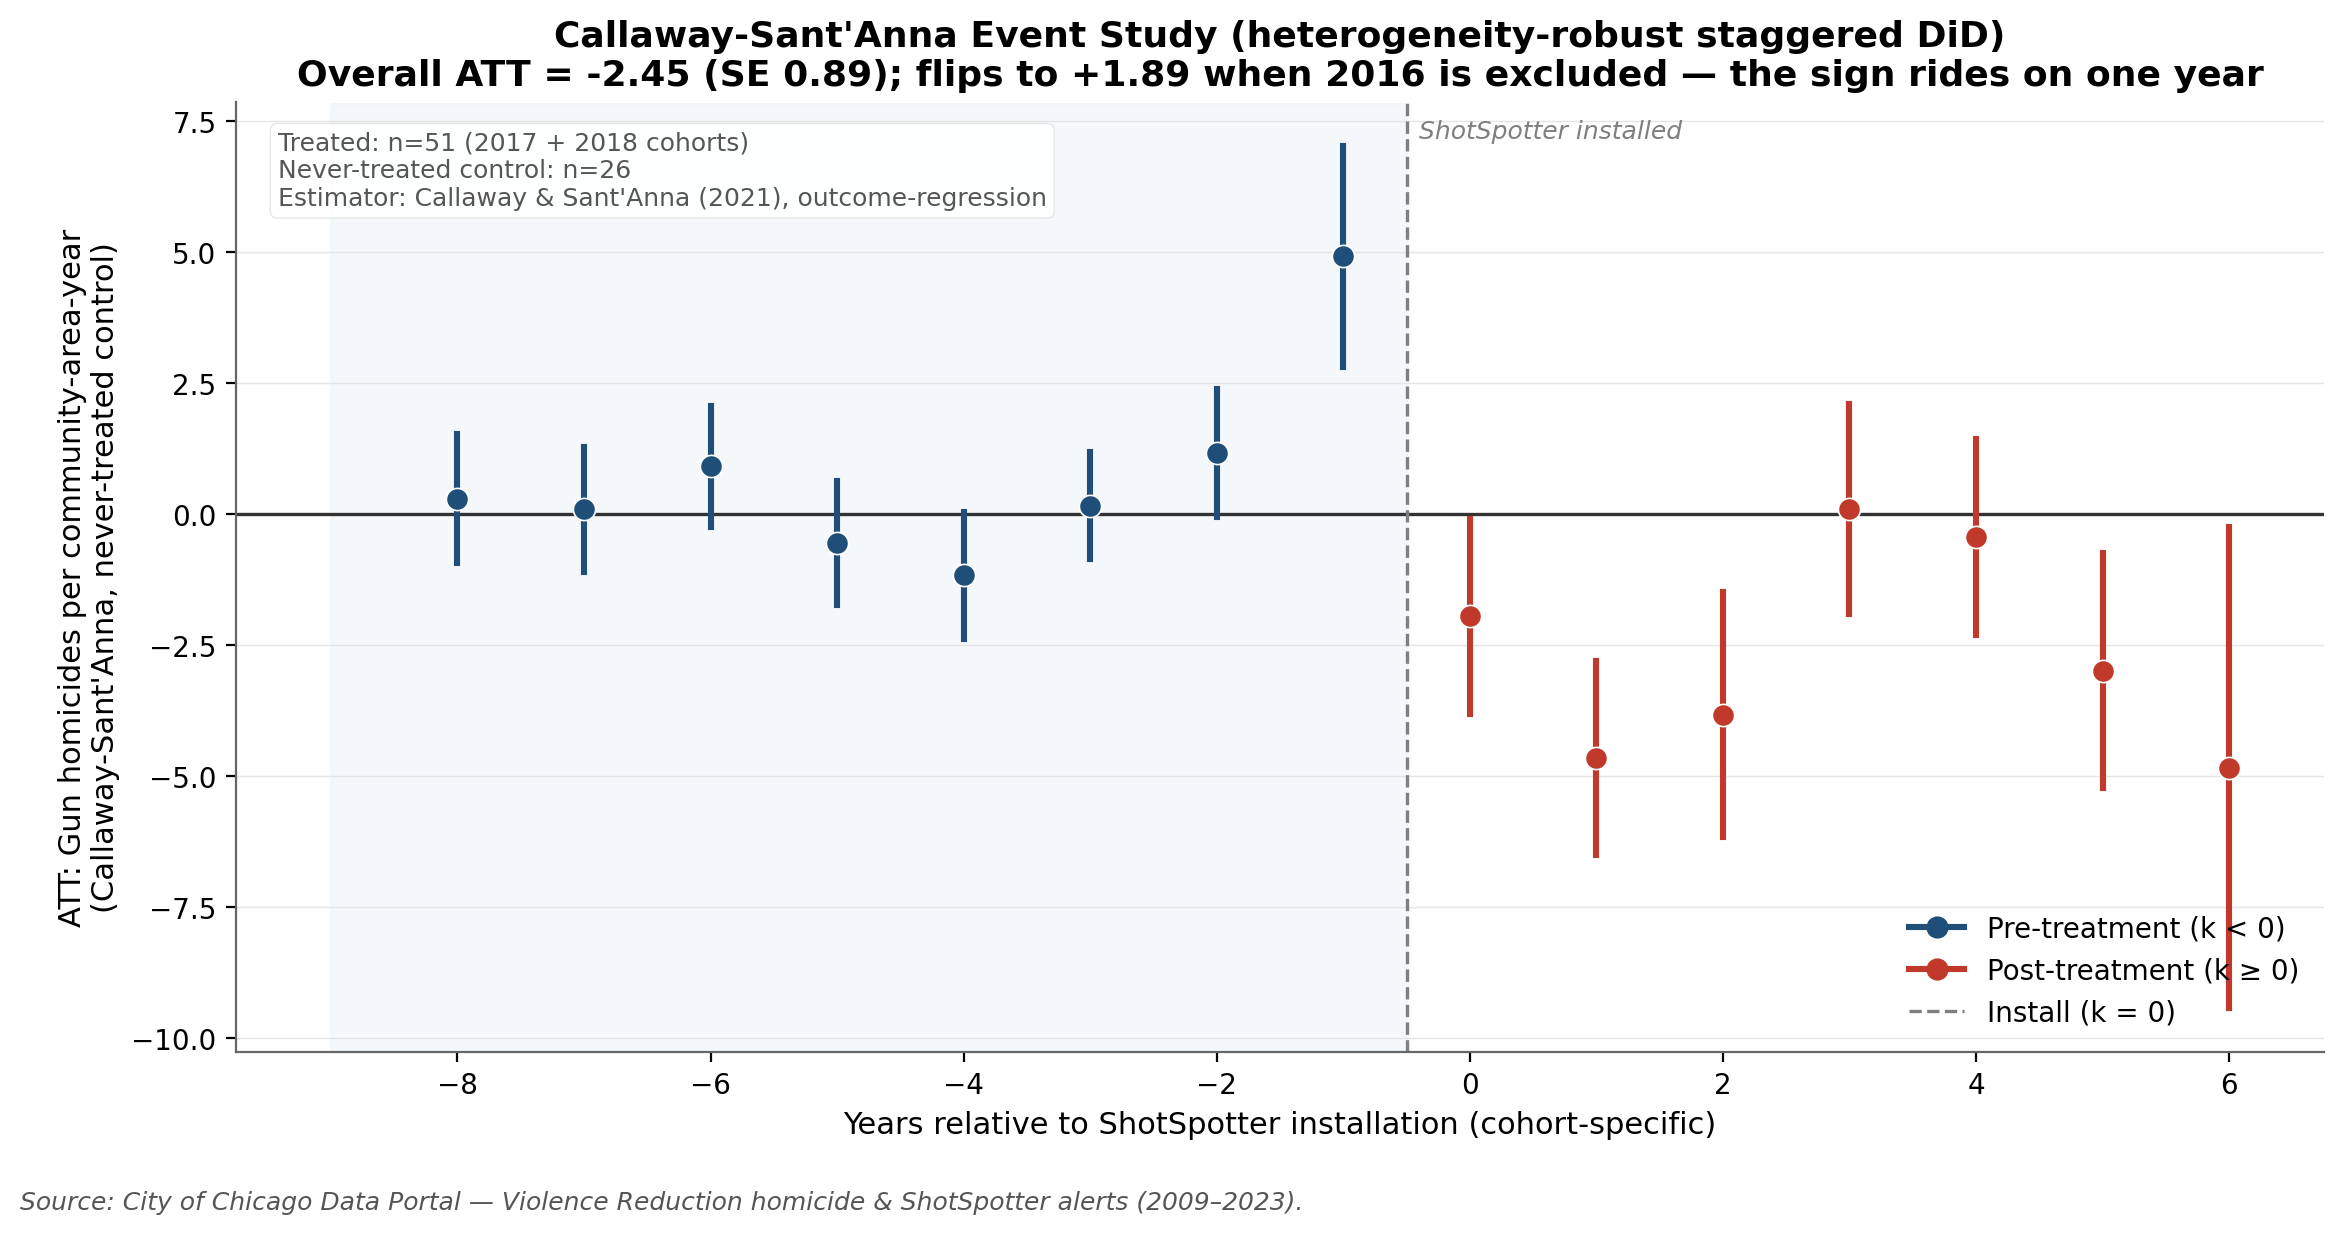
\includegraphics[width=0.85\textwidth]{callaway_santanna_event_study.png}
\caption{Callaway--Sant'Anna heterogeneity-robust event study. The negative overall ATT
rides on the single 2016 pre-coefficient; dropping 2016 flips the overall estimate back
to the sign of OLS.}
\label{fig:cs}
\end{figure}

\begin{figure}[H]
\centering
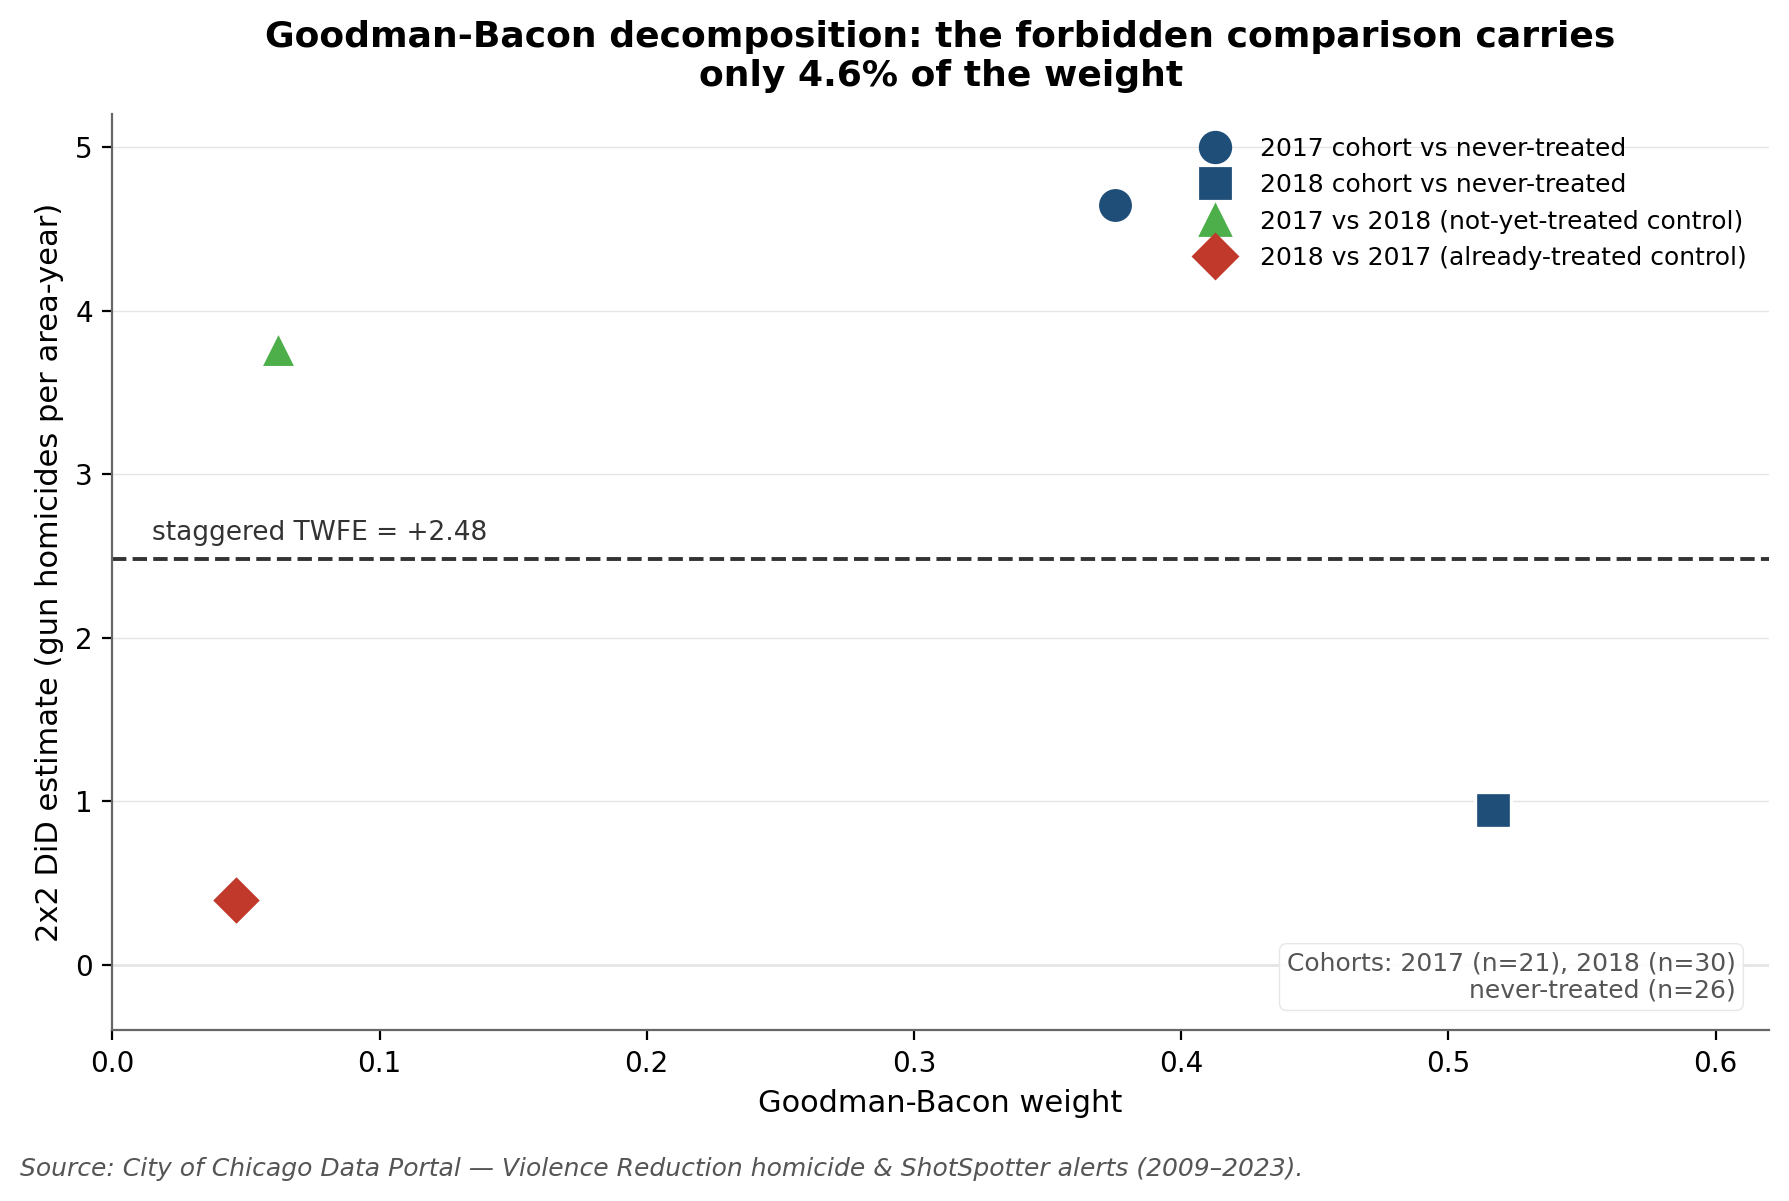
\includegraphics[width=0.8\textwidth]{bacon_decomposition.png}
\caption{Goodman--Bacon decomposition of the staggered TWFE estimate. The ``forbidden''
already-treated comparison (red diamond) carries only 4.6\% of the weight; the weighted
2$\times$2 components reproduce the aggregate coefficient exactly. The estimate's
instability is not staggered-timing contamination.}
\label{fig:bacon}
\end{figure}

\subsection{The selection mechanism: what predicted placement}
\label{sec:placement}

The paper has so far asserted that ShotSpotter was assigned because of pre-existing
violence. Because that selection is the hinge of every identification problem here, we
estimate it directly, modeling ShotSpotter placement across all 77 community areas as a
function of pre-period (2009--2016) gun-homicide levels and the 2008--2012 Census
socioeconomic indicators. One caveat governs the exercise: the city's siting decision was
administrative and made at the police-district level---the OIG documents deployment across
twelve districts---so community-area treatment is the neighborhood-level footprint of that
coarser choice, and the model describes what that footprint tracks, not 77 independent
siting decisions. Two facts emerge. First, placement tracks structural
disadvantage even more tightly than the homicide count itself (Figure~\ref{fig:placement}):
the hardship index separates treated from never-treated areas with an AUC of $0.93$, and
per-capita income and unemployment each with $0.92$, against $0.79$ for the pre-period
gun-homicide count, and
once hardship is held fixed the violence count adds essentially nothing (its coefficient is
statistically insignificant). Violence and disadvantage are entangled---the same
neighborhoods score high on both---so this does not say violence was irrelevant; it says
the city sited ShotSpotter along the map of disinvestment, of which concentrated gun
violence is one facet.

Second, and decisively for identification, placement is nearly deterministic. A propensity
model on pre-period violence, hardship, and income separates the two groups with an AUC of
$0.94$; the median propensity is $0.97$ for ShotSpotter areas against $0.19$ for
never-treated areas; and the six highest-violence study neighborhoods all carry a placement
propensity of at least $0.97$---a band that \emph{no} never-treated area reaches
(Figure~\ref{fig:overlap}). The natural comparison---neighborhoods similar in pre-period
violence that did not receive ShotSpotter---therefore does not exist in Chicago, which is
exactly why the synthetic control below cannot be constructed. This is the selection-side
statement of the counterfactual problem: the city installed ShotSpotter in essentially every highest-violence,
highest-hardship neighborhood, leaving no comparably situated untreated unit from which to
build a counterfactual for the units the study is about.

Placement also mapped onto the city's racial geography. ShotSpotter areas are on average
49\% Black and 32\% Hispanic, against 14\% and 17\% in never-treated areas, and the white,
non-Hispanic share is the single sharpest separator in the whole analysis (13\% versus
56\%, AUC $0.95$). The pattern survives conditioning: adding Black and Hispanic share to the
placement model raises its AUC from $0.94$ to $0.96$, and in a linear-probability model with
pre-period violence, hardship, and income, a one-SD rise in the Black share is associated
with a $+33$ percentage-point change in placement probability ($p = 0.002$) and the Hispanic
share $+28$ points ($p = 0.003$), while violence and hardship themselves turn insignificant.
Race, hardship, and violence are deeply entangled in a segregated city, and with 77 areas the
design cannot separate them cleanly, so this is \emph{not} evidence that race drove siting
independently of disadvantage. What it shows, descriptively, is that ShotSpotter placement
tracked Chicago's racial geography at least as tightly as it tracked violence or hardship.
That coverage blankets the city's highest-Black-and-Latino police districts is already
documented (MacArthur Justice Center, 2021; Office of Inspector General, 2021); our marginal
contribution is the \emph{conditional} result---that racial composition predicts placement
even once pre-period violence and hardship are held fixed. (Community-area race is measured
from the 2019--2023 ACS, which post-dates the rollout; because Chicago's neighborhood racial
composition is highly persistent, we read it as a proxy for the pre-rollout map.)

\begin{figure}[H]
\centering
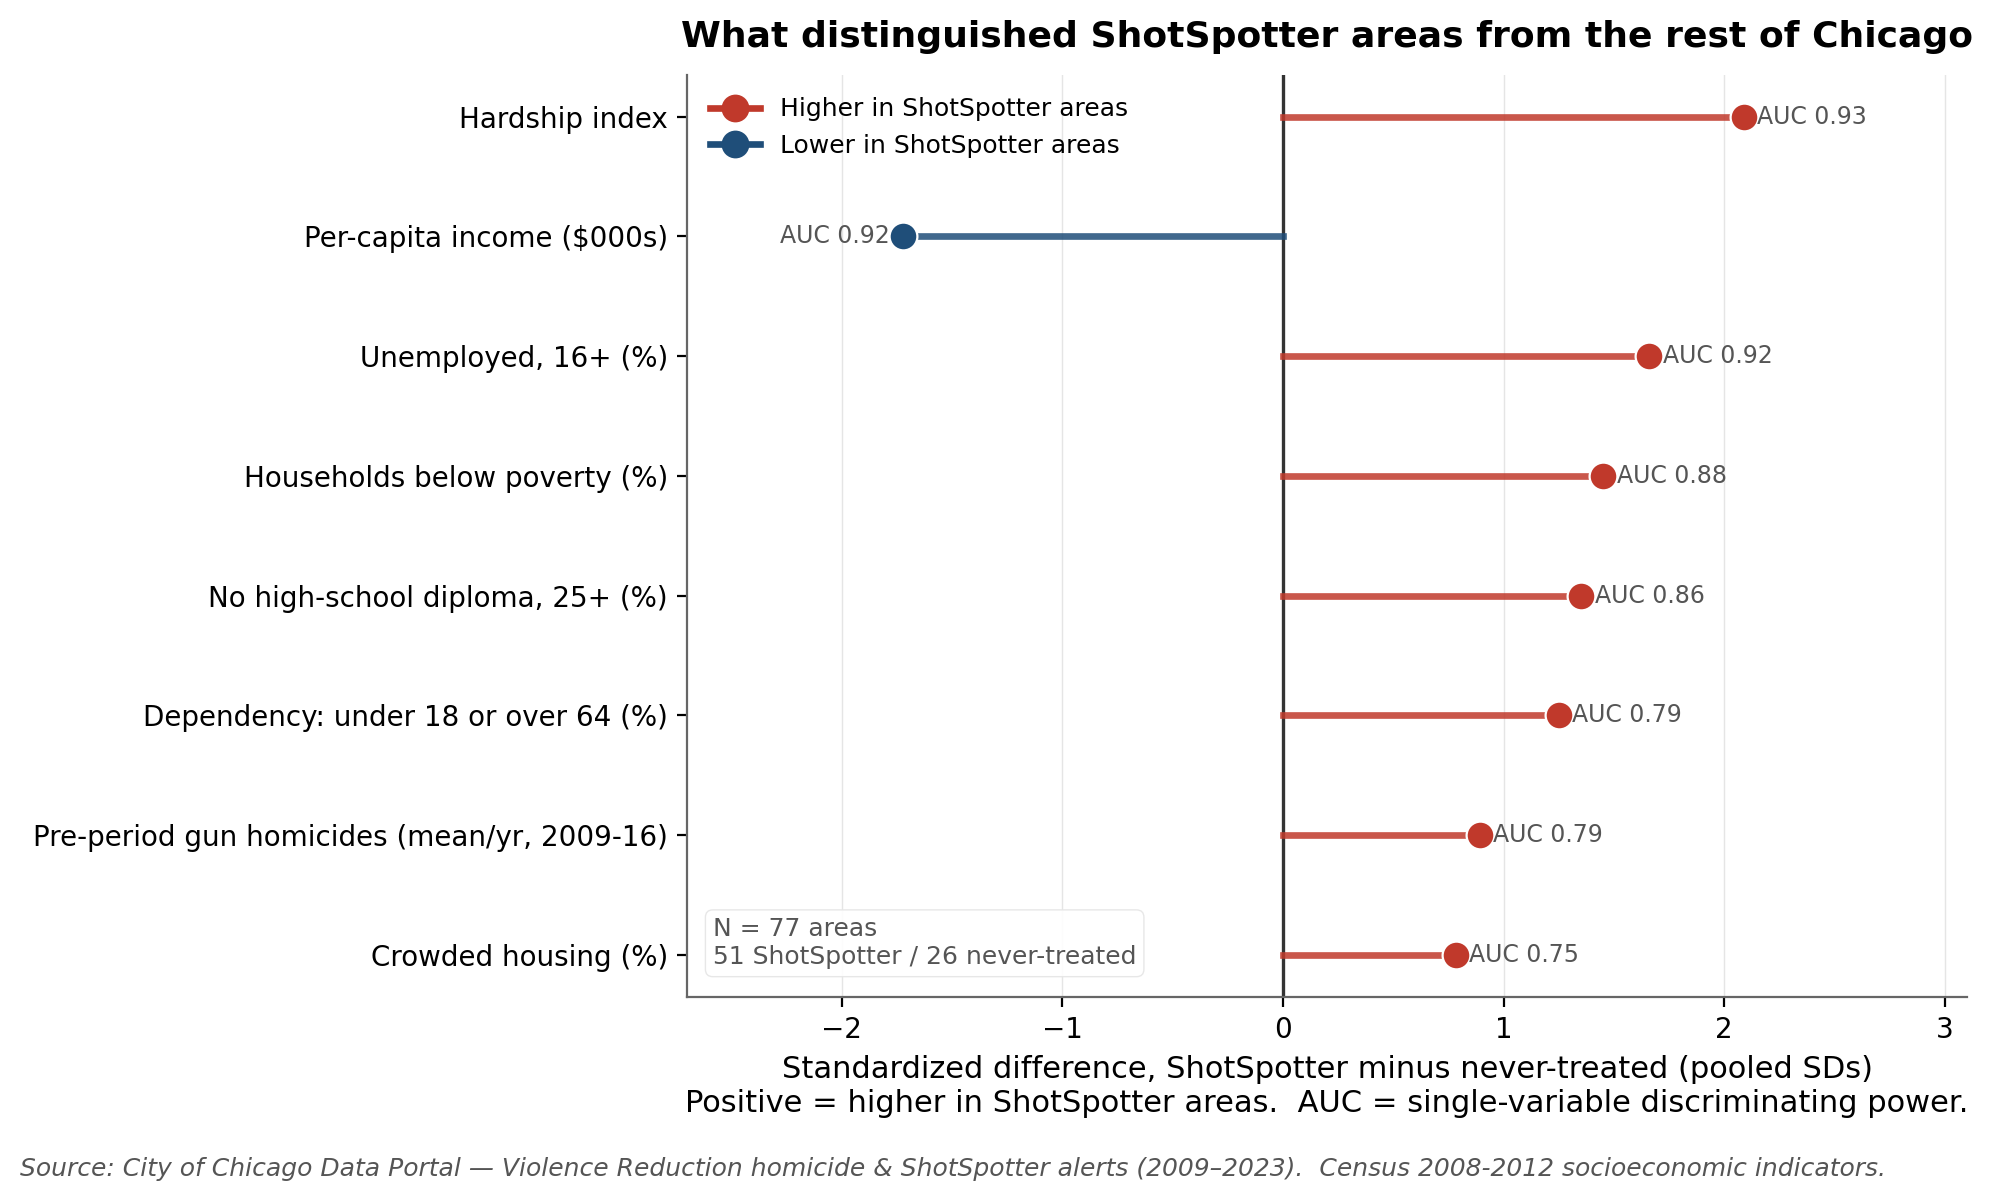
\includegraphics[width=0.85\textwidth]{placement_coefficients.png}
\caption{Standardized differences between ShotSpotter and never-treated community areas on
each characteristic (treated minus control, in pooled SDs), with each variable's
single-predictor discriminating power (AUC). Structural disadvantage---hardship, low
income, unemployment---distinguishes the two groups more sharply than the pre-period
gun-homicide count does.}
\label{fig:placement}
\end{figure}

\begin{figure}[H]
\centering
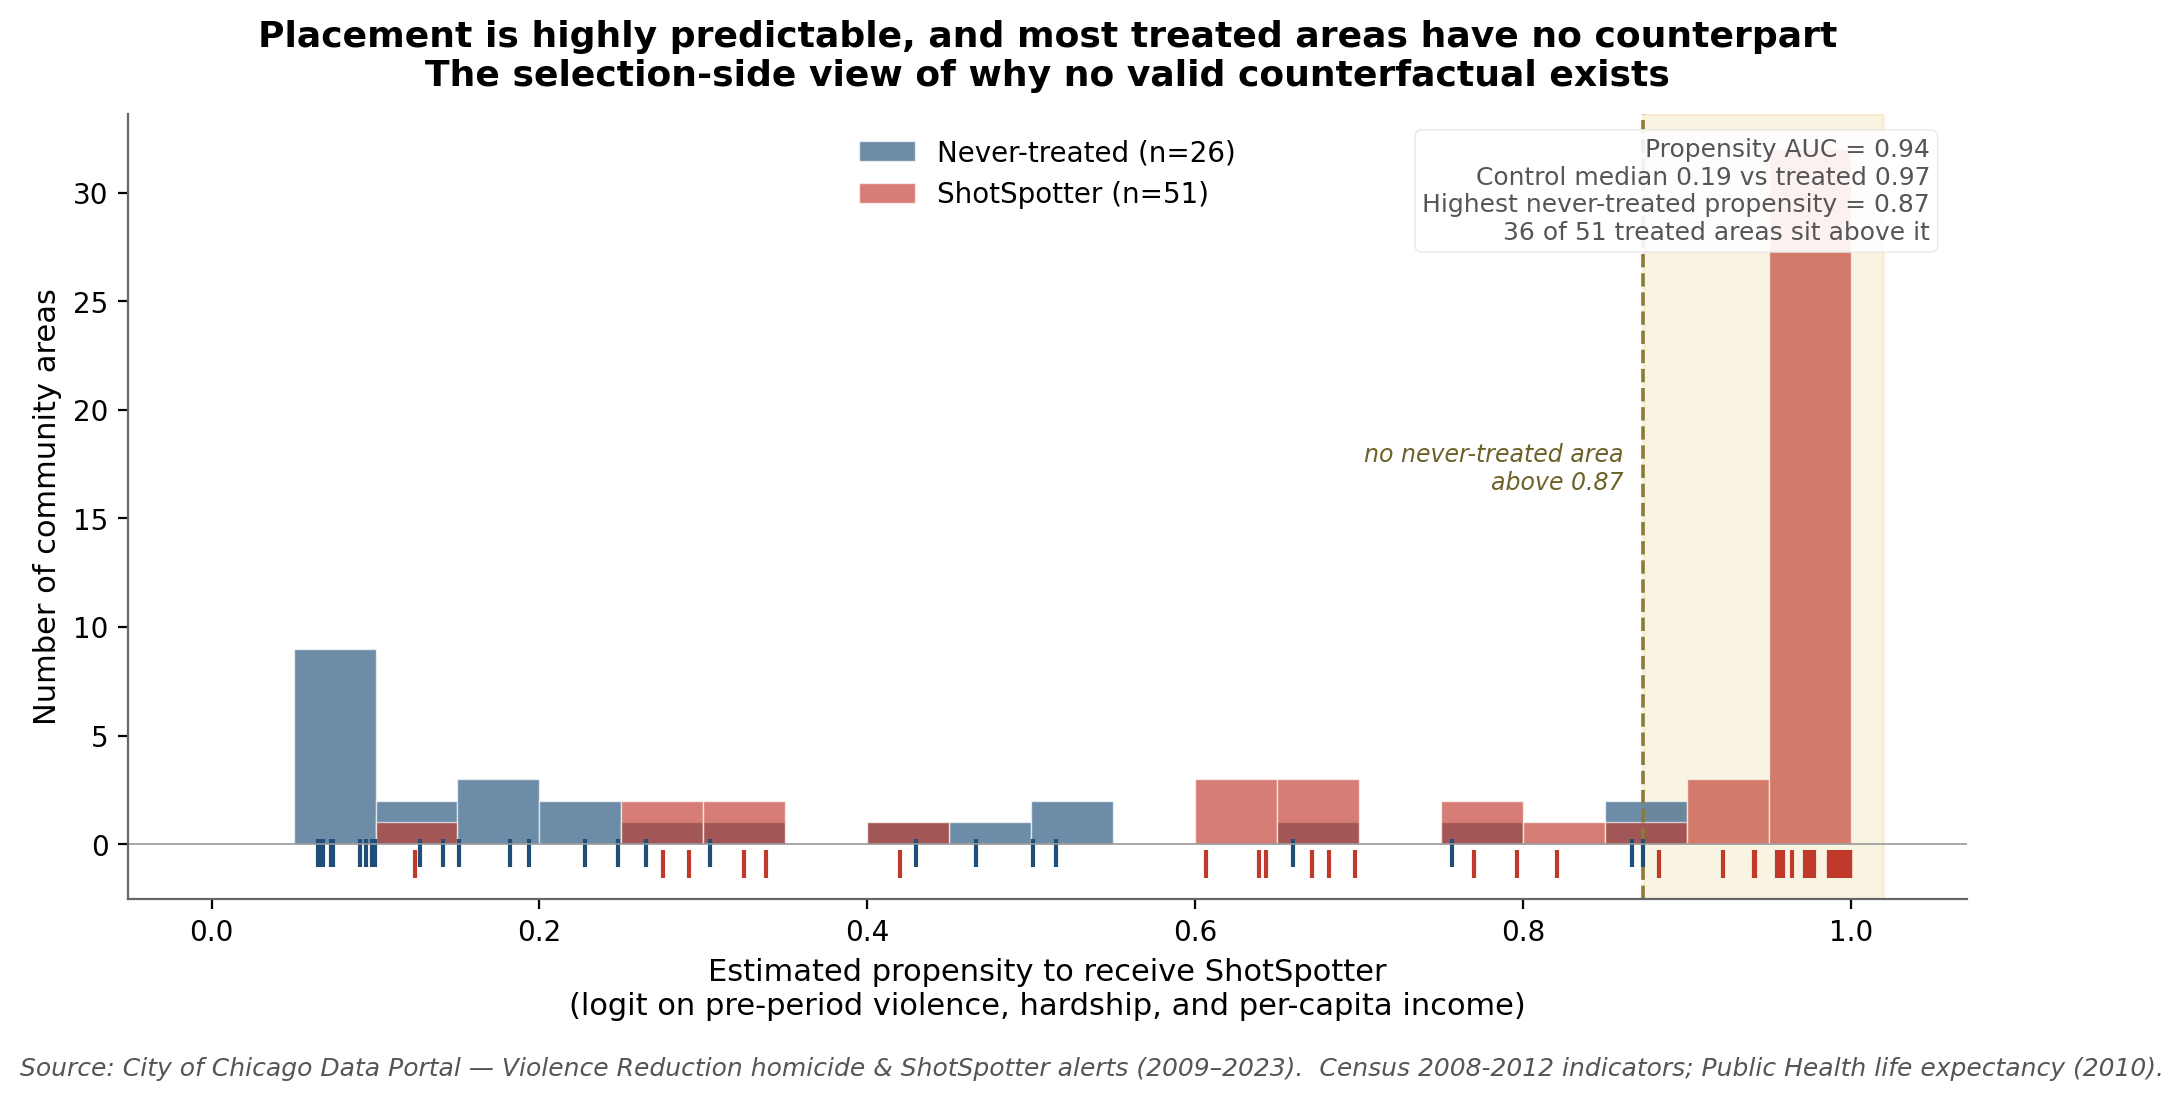
\includegraphics[width=0.85\textwidth]{placement_propensity_overlap.png}
\caption{Estimated propensity to receive ShotSpotter, treated versus never-treated. The
distributions are starkly separated (AUC $0.94$); the shaded band holds the six highest-violence
study neighborhoods (propensity $\geq 0.97$), where no never-treated area appears. Placement
is predictable enough that these units have no untreated counterpart---the selection-side
view of why no valid counterfactual exists.}
\label{fig:overlap}
\end{figure}

\subsection{Synthetic control is infeasible}

For each of the six study neighborhoods, the synthetic-control optimizer concentrates
100\% of the weight on a single donor---Washington Heights, the highest-violence
non-ShotSpotter community area. Pre-treatment RMSEs are large (10--34 homicides per year
against actual values of 15--70), meaning even the best linear combination of donors
cannot reproduce the pre-treatment trajectory of any treated unit. The synthetic
counterfactual lies far below the treated series in every panel of
Figure~\ref{fig:synth}, including in the pre-treatment years it was explicitly fit on.

Permutation inference makes the problem concrete rather than rescuing it. Running the
same synthetic control on each of the 26 never-treated areas produces a tight placebo-gap
distribution centered near zero against actual treated gaps of $+14$ to $+49$; the naive
permutation $p$-value is below $0.001$ for every treated unit. But this rejection is
\emph{invalid by construction}: it is dominated by the level mismatch between treated and
donor units, not by any treatment effect. The 26 never-treated community areas occupy the
low-violence end of Chicago's distribution, so there is no donor pool capable of
constructing a credible counterfactual for the city's most violent neighborhoods. This
is not a failure of method; it is a feature of the data. ShotSpotter's selection
rule---deploy where violence is highest---is, in a literal sense, what makes synthetic
control infeasible. The absence of a counterfactual is itself the finding.

The contrast with settings where synthetic control \emph{does} work is instructive. In
Kansas City, gunshot detection covers a localized 3.5-square-mile zone---about 1\% of the
city---leaving a large donor pool of untreated micro-units, and a microsynthetic control
is feasible (Piza et al., 2024; Robbins \& Davenport, 2021). Chicago is the mirror image:
coverage blankets essentially every high-violence community area, so the pool of comparably
violent untreated donors is empty. Infeasibility here is therefore not a shortcoming of the
estimator but a consequence of near-universal treatment among the units of interest---the
same fact the placement model states from the selection side. Permutation $p$-values from
synthetic control lack a clean interpretation in any case (Ferman et al., 2020).

\begin{figure}[H]
\centering
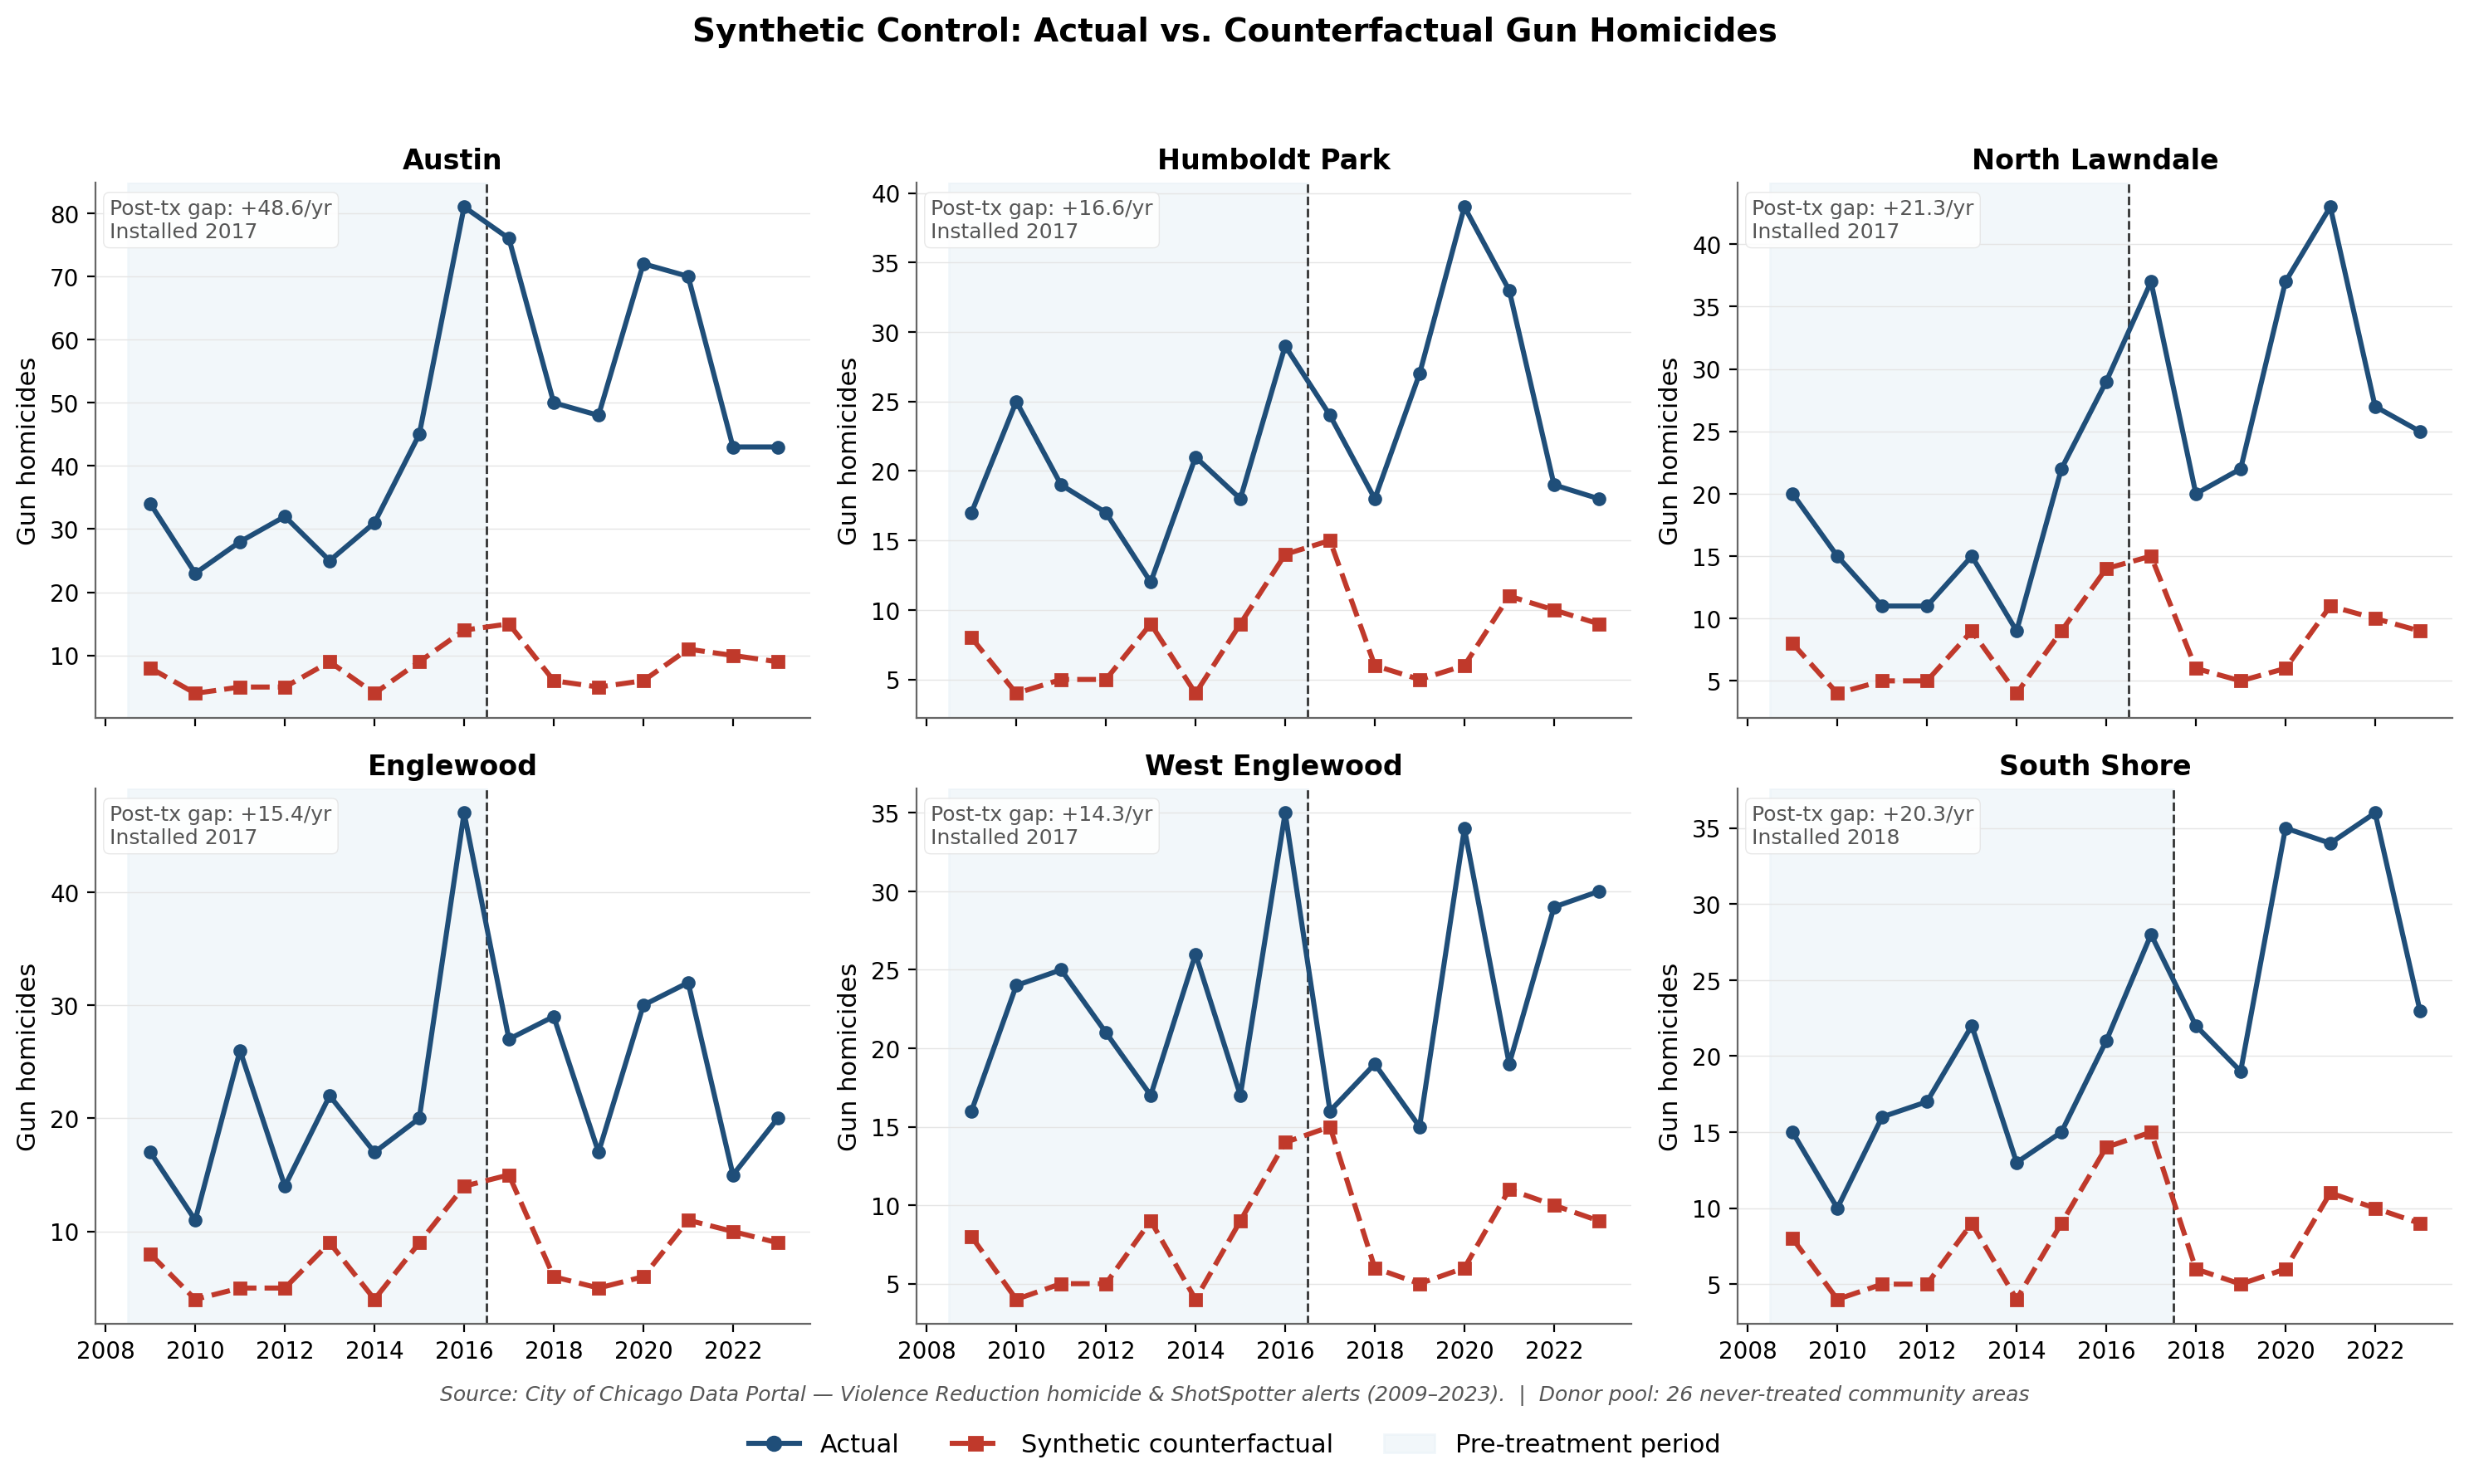
\includegraphics[width=\textwidth]{synthetic_control_panels.png}
\caption{Synthetic control for the six study neighborhoods. The synthetic counterfactual
(red) sits far below the actual series (blue) even in the pre-treatment window it was fit
on, because no combination of the 26 lower-violence never-treated areas can match a
high-violence treated unit. The method is infeasible for these data.}
\label{fig:synth}
\end{figure}

\subsection{What does explain neighborhood-level violence?}

The hardship index from the 2008--2012 Census ranks the six study neighborhoods at 55,
73, 85, 87, 89, and 94---against a city-wide hardship score below 50 and the
lowest-violence community areas at 1--10. Per-capita income in these neighborhoods ranges
from about \$11,000 to \$19,000, against a city-wide \$28,202. The same neighborhoods
that had the highest homicide rates \emph{before} ShotSpotter still had the highest
homicide rates after. Cross-sectional variation in violence tracks structural
disadvantage tightly; cross-sectional variation in ShotSpotter coverage adds little
explanatory power once disadvantage is held constant.

% ===========================================================================
\section{What the Data Can and Cannot Support}

Taken together---(a) an OLS DiD coefficient that disappears under proper count-data
regression (Poisson IRR $1.07$, $p = 0.51$; Negative Binomial IRR $1.07$, $p = 0.55$);
(b) a Wald $F$-test that rejects parallel trends at the 1\% level ($F = 19.9$, $p =
0.006$); (c) similarly significant pre-period placebos; (d) an infeasible synthetic
control; and (e) a Callaway--Sant'Anna estimate whose sign reverses ($-2.45$ to $+1.90$)
when one anomalous year is dropped---the evidence points to a single conclusion: \textbf{the
design cannot credibly identify the causal effect of ShotSpotter installation on gun
homicides.} Table~\ref{tab:summary} lays out why the estimators differ.

\begin{table}[H]
\centering
\small
\caption{Why the estimates differ---and what actually moves each one.}
\label{tab:summary}
\begin{tabular}{p{0.30\textwidth}p{0.22\textwidth}p{0.40\textwidth}}
\toprule
Estimator & Full panel & What actually moves it \\
\midrule
Naive OLS DiD & $+2.63$ ($p < 0.001$) & Additive scale, inflated by high-count areas \\
Poisson / Neg.\ Binomial & IRR $\approx 1.07$ (ns) & Positive in sign, but null on the multiplicative scale \\
Callaway--Sant'Anna & $-2.45$ ($p < 0.01$) & Flips to $+1.90$ once the 2016 outlier year is dropped \\
\bottomrule
\end{tabular}
\end{table}

The data do not say ShotSpotter caused a 2.6-homicide-per-year \emph{increase}---that
statistic is a misspecification artifact. Neither do they say it caused a reduction---that
reading takes a 2016-driven event-study coefficient too literally. The proper count-data
specifications return statistically null effects with confidence intervals spanning the
entire policy-relevant range.

We can, however, bound the answer in one direction: \textbf{the data are inconsistent with
a large \emph{deterrence} effect}---a broad, sustained fall in the number of shootings of
the kind detection volume alone was meant to produce. A treatment that large, at these
sample sizes, would have produced visibly negative post-treatment event-study coefficients
with intervals excluding zero, robustness across specifications, and a cleaner signal in
the higher-powered non-fatal-shootings analysis. None of these appear.

What the design cannot rule out is a benefit operating through a different channel. A
boundary regression-discontinuity analysis attributes roughly 85 fewer deaths per year to
faster emergency response inside coverage, working through victim survival rather than
deterrence (University of Chicago Crime Lab, 2024; a working analysis, not yet
peer-reviewed). The direct tests of that channel are equivocal rather than supportive: the
two studies that measured case fatality found no reduction---Piza et al.\ (2024) compare
the fatal and non-fatal shooting counts in the Kansas City coverage area and find no
difference, and a Camden trauma-registry study found faster prehospital times but no
significant adjusted mortality difference, albeit among more severely injured detected
victims (Goldenberg et al., 2019). The mechanism is real---detection alerts precede the
first 911 call by a median of roughly 90 seconds (Piza et al., 2023)---but its translation
into fewer deaths is unproven. A mortality reduction of the magnitude the discontinuity
implies would still fall \emph{inside} our own count-model confidence interval, and a community-area-by-year homicide panel---which
observes neither response times nor the conversion of shootings into deaths---is simply not
built to detect it. Ruling out a large deterrence effect is therefore not the same as
ruling out every benefit, and we do not claim the stronger statement. Whatever effect
ShotSpotter had on gun homicides through deterrence was not large enough to dominate the
noise, the 2016 anomaly, or the pre-existing trend differences across neighborhoods, and it
falls far short of the reduction a \$3 million detection contract was meant to deliver.

% ===========================================================================
\section{Why Detection Would Not Be Expected to Reduce Violence}

Three explanations are consistent with this empirical pattern.

\textbf{Selection.} ShotSpotter was installed in the places that needed it most. Even if
the technology produced a small benefit, the comparison would still look unfavorable
because the rest of Chicago started from a much lower baseline with less room to
deteriorate.

\textbf{Detection is not intervention.} The mechanism by which ShotSpotter could
plausibly reduce homicides runs through faster police response and faster trauma triage.
The data here do not measure response times, dispatch decisions, or trauma outcomes, and
the 2021 OIG audit found that alerts rarely produced investigative evidence and that
officer behavior did not consistently change in response to alerts (Office of Inspector
General, 2021; Thompson, Lawrence, \& La Vigne, 2020). If the operational link between
detection and outcome is weak, detection volume is not a sufficient condition for fewer
homicides.

\textbf{Structural factors dominate.} A surveillance technology cannot, by itself, change
the distribution of poverty, unemployment, housing instability, or labor-market access.
Programs that have reduced homicide in randomized or quasi-experimental
evaluations---READI Chicago, Cure Violence, Becoming a Man---work on those structural
channels directly. A microphone on a streetlight does not.

% ===========================================================================
\section{Limitations}

The most important limitation is the one developed throughout the paper: the design
itself cannot identify a clean treatment effect from these data, because the city did not
generate the counterfactual we need---Chicago neighborhoods with ShotSpotter-eligible
violence levels but no ShotSpotter installation. Beyond that, several caveats are worth
naming explicitly. The unit of analysis is coarse. The crime-and-place literature favors
micro-geographic units---street segments---over administrative geographies (Weisburd, 2015),
and Schnell, Braga, and Piza (2017) show for Chicago specifically that community areas mask
within-area heterogeneity that finer units capture; evaluations pinned to administrative
units can also overstate coverage (Doucette et al., 2021). We use the community area
deliberately, because it is the unit at which Chicago's open data are published and its
policy debate is conducted, and the paper's claim is precisely that at this policy-grade
resolution the effect is not identifiable---the coarseness is part of the finding, not an
assumption to wave away. A micro-geographic re-estimation, once the city releases the
sensor-coverage polygons, would be the natural complement. The panel is annual, masking
within-year dynamics. Standard errors
cluster on community area (about 77 clusters); a restricted wild-cluster bootstrap
(Cameron, Gelbach, \& Miller, 2008; 999 Rademacher replications) returns $p \approx
0.001$ for the OLS DiD in every specification, so the headline coefficient is not an
artifact of thin-cluster inference---the problem is the specification and the design,
not the standard errors. Two event-study implementations
are reported---a transparent hand-rolled difference-in-means kept for intuition, and the
packaged Callaway--Sant'Anna estimator, which should be treated as the authoritative
staggered-DiD result. The placement model is cross-sectional and descriptive: it documents
the selection pattern but does not identify a causal siting rule, and its racial-composition
measure is drawn from the 2019--2023 ACS, a proxy for the pre-rollout composition that
relies on the persistence of Chicago's neighborhood racial geography. A subtler caveat
applies to the count models that carry the headline null: the Poisson and Negative Binomial
DiD use two-way fixed effects, and under a staggered rollout a two-way fixed-effects PPML
inherits the same heterogeneity-weighting problem as linear TWFE, placing potentially
negative weights on some treated cells (Moreau-Kastler, 2025). The heterogeneity-robust
estimator we do report---Callaway--Sant'Anna---is linear and does not transfer to the
multiplicative outcome the count argument itself calls for; the appropriate tool is a
nonlinear, heterogeneity-robust count estimator (Wooldridge, 2023; Moreau-Kastler, 2025),
which we leave to follow-up. This does not rescue a causal reading---if anything it is one
more reason the effect is not cleanly identified---but the reported incidence-rate ratio is
best read as a pooled two-way-FE summary, not a heterogeneity-robust ATT. And the analysis
observes neither police response times, dispatch decisions, nor arrests---the actual channel
through which detection could plausibly reduce violence.

The comparison a credible design needs---similarly violent places without detection---must
therefore be built outside the community-area frame, and the existing literature shows how:
Connealy et al. (2024) construct it by matching Chicago police districts, and Doucette et
al. (2021) by comparing metropolitan counties nationally; both recover the null this panel
cannot identify. Within Chicago, three designs would do better with data the city has not
released: a geographic regression discontinuity at sensor-coverage boundaries (which
requires the unreleased coverage polygons), estimation at census-tract-by-month resolution,
and direct measurement of the response-time mechanism around each activation date.

% ===========================================================================
\section{Conclusion}

ShotSpotter in Chicago succeeded at detection: alerts climbed in covered areas because
the technology measures gunfire that 911 calls underreport. What cannot be demonstrated
is that detection translated into a reduction in lethal violence. Every design we ran on
these data either produces a positive DiD coefficient that fails falsification and
collapses under proper count-data modeling, an event study that violates parallel trends
because of the 2016 anomaly, or a synthetic control whose donor pool cannot match
treated-area violence levels. With no valid control group and a pre-period dominated by
one outlier year, these data simply cannot identify a causal effect in either direction.
They are inconsistent with a large \emph{deterrence} effect, though not with the smaller,
survival-channel mortality benefit a boundary discontinuity design attributes to faster
response---an effect this panel is not built to see.

That non-result is itself a policy statement. The 2023 termination of Chicago's
ShotSpotter contract is consistent with the absence, in the aggregate data, of the broad
violence reduction the technology was marketed to deliver. Resources reallocated from
detection contracts toward community-based violence-prevention programs---READI Chicago,
Cure Violence, Becoming a Man---would, on the existing quasi-experimental evidence, have at
least as good a chance of producing the homicide reductions ShotSpotter has not been shown
to deliver at scale. Technology can help detect the problem; on this evidence, it has not
been shown to solve it.

% ===========================================================================
\section*{Data and Code Availability}

Every input is a public product of the City of Chicago Data Portal
(\url{https://data.cityofchicago.org}): Violence Reduction---Victims of Homicides and
Non-Fatal Shootings (\texttt{gumc-mgzr}); Violence Reduction---ShotSpotter Alerts
(Historical) (\texttt{3h7q-7mdb}); Census Data---Selected Socioeconomic Indicators,
2008--2012 (\texttt{kn9c-c2s2}); ACS 5-Year Data by Community Area (\texttt{t68z-cikk}); and
the Community Areas boundary file (\texttt{cauq-8yn6}). The complete analysis
pipeline---data-processing, all five estimator classes, the placement model, and every
figure---is openly available and reproduces the paper end to end at
\url{https://github.com/abelma2/ACE592_Final_Project}.

% ===========================================================================
\singlespacing
\section*{References}
\begin{flushleft}
\setlength{\parindent}{-0.5in}
\leftskip=0.5in

Abadie, A., Diamond, A., \& Hainmueller, J. (2010). Synthetic control methods for
comparative case studies: Estimating the effect of California's tobacco control program.
\emph{Journal of the American Statistical Association, 105}(490), 493--505.

Bertrand, M., Duflo, E., \& Mullainathan, S. (2004). How much should we trust
differences-in-differences estimates? \emph{Quarterly Journal of Economics, 119}(1),
249--275.

Braga, A. A., \& Cook, P. J. (2023). \emph{Policing gun violence: Strategic reforms for
controlling our most pressing crime problem}. Oxford University Press.

Callaway, B., \& Sant'Anna, P. H. C. (2021). Difference-in-differences with multiple time
periods. \emph{Journal of Econometrics, 225}(2), 200--230.

Cameron, A. C., Gelbach, J. B., \& Miller, D. L. (2008). Bootstrap-based improvements for
inference with clustered errors. \emph{Review of Economics and Statistics, 90}(3),
414--427.

Cameron, A. C., \& Trivedi, P. K. (2013). \emph{Regression analysis of count data} (2nd
ed.). Cambridge University Press.

Carr, J., \& Doleac, J. L. (2016). The geography, incidence, and underreporting of gun
violence: New evidence using ShotSpotter data. Working paper.

Centers for Disease Control and Prevention (CDC). (2020). \emph{Firearm mortality by
state and demographic group---United States, 2018}.
\url{https://www.cdc.gov/nchs/pressroom/states/illinois/il.htm}

Choi, K. S., Librett, M., \& Collins, T. J. (2014). An empirical evaluation: Gunshot
detection system and its effectiveness on police practices. \emph{Police Practice and
Research, 15}(1), 48--61.

Connealy, N. T., Piza, E. L., Arietti, R. A., Carter, J. G., \& Mohler, G. (2024).
Staggered deployment of gunshot detection technology in Chicago, IL: A matched
quasi-experiment of gun violence outcomes. \emph{Journal of Experimental Criminology,
20}(4), 1027--1053.

de Chaisemartin, C., \& D'Haultf\oe uille, X. (2020). Two-way fixed effects estimators with
heterogeneous treatment effects. \emph{American Economic Review, 110}(9), 2964--2996.

Doucette, M. L., Green, C., Necci Dineen, J., Shapiro, D., \& Raissian, K. M. (2021).
Impact of ShotSpotter technology on firearm homicides and arrests among large
metropolitan counties: A longitudinal analysis, 1999--2016. \emph{Journal of Urban
Health, 98}(5), 609--621.

Ferman, B., Pinto, C., \& Possebom, V. (2020). Cherry picking with synthetic controls.
\emph{Journal of Policy Analysis and Management, 39}(2), 510--532.

Gatens, A., \& Reichert, J. (2019). \emph{Police technology: Acoustic gunshot detection
systems}. Illinois Criminal Justice Information Authority.

Goldenberg, A., Rattigan, D., Dalton, M., Gaughan, J. P., Thomson, J. S., Remick, K.,
Butts, C., \& Hazelton, J. P. (2019). Use of ShotSpotter detection technology decreases
prehospital time for patients sustaining gunshot wounds. \emph{Journal of Trauma and Acute
Care Surgery, 87}(6), 1253--1259.

Goodman-Bacon, A. (2021). Difference-in-differences with variation in treatment timing.
\emph{Journal of Econometrics, 225}(2), 254--277.

Harcourt, B. E. (2019). \emph{Against prediction: Profiling, policing, and punishing in
an actuarial age}. University of Chicago Press.

Huff, J., Dunlap, B., \& Pearson, R. L., Jr. (2026). Does acoustic gunshot detection
technology reduce crime? A systematic review and meta-analysis. \emph{American Journal of
Criminal Justice}. Advance online publication.

Irvin-Erickson, Y., Bai, B., Gurvis, A., \& Mohr, E. (2016). \emph{The effect of gun
violence on local economies}. Urban Institute.

Kegler, S. R., Dahlberg, L. L., \& Mercy, J. A. (2018). Firearm homicides and suicides in
major metropolitan areas---United States, 2012--2013 and 2015--2016. \emph{Morbidity and
Mortality Weekly Report, 67}.

LaLonde, R. J. (1986). Evaluating the econometric evaluations of training programs with
experimental data. \emph{American Economic Review, 76}(4), 604--620.

MacArthur Justice Center. (2021). \emph{ShotSpotter generated over 40,000 dead-end police
deployments in Chicago in 21 months, according to new study}. Northwestern Pritzker School
of Law.

Mares, D. (2023). Evaluating an acoustic gunshot detection system in Cincinnati. In E. R.
Groff \& C. P. Haberman (Eds.), \emph{Understanding crime and place: A methods handbook}
(pp. 396--406). Temple University Press.

Mares, D., \& Blackburn, E. (2021). Acoustic gunshot detection systems: A quasi-experimental
evaluation in St.\ Louis, MO. \emph{Journal of Experimental Criminology, 17}(2), 193--215.

Moreau-Kastler, N. (2025). \emph{Proportional treatment effects in staggered settings: An
approach for Poisson pseudo-maximum likelihood}. Working paper, Sciences Po.

Office of Inspector General, City of Chicago. (2021, August 24). \emph{The Chicago Police
Department's use of ShotSpotter technology}.
\url{https://www.chicago.gov/content/dam/city/depts/oig/publications/reports-public-safety/2021/CPD-ShotSpotter-Report-8-24-21.pdf}

Piza, E. L., Hatten, D. N., Carter, J. G., Baughman, J. H., \& Mohler, G. O. (2023).
Gunshot detection technology time savings and spatial precision: An exploratory analysis in
Kansas City. \emph{Policing: A Journal of Policy and Practice, 17}, paac097.

Piza, E. L., Hatten, D. N., Mohler, G. O., Carter, J. G., \& Cho, J. (2024). Gunshot
detection technology effect on gun violence in Kansas City, Missouri: A microsynthetic
control evaluation. \emph{Criminology \& Public Policy, 23}, 863--892.

Raphael, S., \& Stoll, M. A. (2013). \emph{Why are so many Americans in prison?} Russell
Sage Foundation.

Robbins, M. W., \& Davenport, S. (2021). microsynth: Synthetic control methods for
disaggregated and micro-level data in R. \emph{Journal of Statistical Software, 97}(2).

Roth, J. (2022). Pretest with caution: Event-study estimates after testing for parallel
trends. \emph{American Economic Review: Insights, 4}(3), 305--322.

Santos Silva, J. M. C., \& Tenreyro, S. (2006). The log of gravity. \emph{Review of
Economics and Statistics, 88}(4), 641--658.

Schnell, C., Braga, A. A., \& Piza, E. L. (2017). The influence of community areas,
neighborhood clusters, and street segments on the spatial variability of violent crime in
Chicago. \emph{Journal of Quantitative Criminology, 33}(3), 469--496.

Thompson, P. S., Lawrence, D. S., \& La Vigne, N. G. (2020). Securing officer buy-in when
a beneficial technology increases workload: Best practices for implementing gunshot
detection technology. \emph{ACJS Today, 46}(1), 1--7.

Topper, M., \& Ferrazares, T. (2024). The unintended consequences of policing technology:
Evidence from ShotSpotter. Forthcoming, \emph{Journal of Human Resources} (SSRN 4828813).

University of Chicago Crime Lab. (2024). Op-ed and replication analysis of ShotSpotter and
shooting fatality in Chicago [not peer-reviewed]. Replication code:
\url{https://github.com/uchicago-urbanlabs-crimelab/shotspotter-op-ed}.

Vovak, H., Riddle, T., Taniguchi, T., Hoogesteyn, K., \& Yang, Y. (2021). \emph{Strategies
for Policing Innovation (SPI) in Wilmington, Delaware: Targeting violent crime} [Final
evaluation report]. National Police Foundation.

Weisburd, D. (2015). The law of crime concentration and the criminology of place.
\emph{Criminology, 53}(2), 133--157.

Wilson, D. B. (2022). The relative incident rate ratio effect size for count-based impact
evaluations: When an odds ratio is not an odds ratio. \emph{Journal of Quantitative
Criminology, 38}(2), 323--341.

Wooldridge, J. M. (2023). Simple approaches to nonlinear difference-in-differences with
panel data. \emph{The Econometrics Journal, 26}(3), C31--C66.

\end{flushleft}

\end{document}
